%% This is file `elsarticle-template-1-num.tex',a
%%
%% Copyright 2009 Elsevier Ltd
%%
%% This file is part of the 'Elsarticle Bundle'.
%% ---------------------------------------------
%%
%% It may be distributed under the conditions of the LaTeX Project Public
%% License, either version 1.2 of this license or (at your option) any
%% later version.  The latest version of this license is in
%%    http://www.latex-project.org/lppl.txt
%% and version 1.2 or later is part of all distributions of LaTeX
%% version 1999/12/01 or later.
%%
%% The list of all files belonging to the 'Elsarticle Bundle' is
%% given in the file `manifest.txt'.
%%
%% Template article for Elsevier's document class `elsarticle'
%% with numbered style bibliographic references
%%
%% $Id: elsarticle-template-1-num.tex 149 2009-10-08 05:01:15Z rishi $
%% $URL: http://lenova.river-valley.com/svn/elsbst/trunk/elsarticle-template-1-num.tex $
%%
\documentclass[preprint,12pt]{elsarticle}
\usepackage{amsmath}
\usepackage{graphicx,subcaption}
\usepackage{listings}
\usepackage{hyperref}
\usepackage{multirow}
\usepackage{notoccite}
\hypersetup{
    colorlinks,
    citecolor=black,
    filecolor=black,
    linkcolor=black,
    urlcolor=black
}

%% Use the option review to obtain double line spacing
%% \documentclass[preprint,review,12pt]{elsarticle}

%% Use the options 1p,twocolumn; 3p; 3p,twocolumn; 5p; or 5p,twocolumn
%% for a journal layout:
%% \documentclass[final,1p,times]{elsarticle}
%% \documentclass[final,1p,times,twocolumn]{elsarticle}
%% \documentclass[final,3p,times]{elsarticle}
%% \documentclass[final,3p,times,twocolumn]{elsarticle}
%% \documentclass[final,5p,times]{elsarticle}
%% \documentclass[final,5p,times,twocolumn]{elsarticle}

%% if you use PostScript figures in your article
%% use the graphics package for simple commands
%% \usepackage{graphics}
%% or use the graphicx package for more complicated commands
%% \usepackage{graphicx}
%% or use the epsfig package if you prefer to use the old commands
%% \usepackage{epsfig}

%% The amssymb package provides various useful mathematical symbols
\usepackage{amssymb}
%% The amsthm package provides extended theorem environments
%% \usepackage{amsthm}

%% The lineno packages adds line numbers. Start line numbering with
%% \begin{linenumbers}, end it with \end{linenumbers}. Or switch it on
%% for the whole article with \linenumbers after \end{frontmatter}.
\usepackage{lineno}

%% natbib.sty is loaded by default. However, natbib options can be
%% provided with \biboptions{...} command. Following options are
%% valid:

%%   round  -  round parentheses are used (default)
%%   square -  square brackets are used   [option]
%%   curly  -  curly braces are used      {option}
%%   angle  -  angle brackets are used    <option>
%%   semicolon  -  multiple citations separated by semi-colon
%%   colon  - same as semicolon, an earlier confusion
%%   comma  -  separated by comma
%%   numbers-  selects numerical citations
%%   super  -  numerical citations as superscripts
%%   sort   -  sorts multiple citations according to order in ref. list
%%   sort&compress   -  like sort, but also compresses numerical citations
%%   compress - compresses without sorting
%%
%% \biboptions{comma,round}

% \biboptions{}

\let\originaleqref\eqref
\renewcommand{\eqref}{Eq.~\originaleqref}

\hypersetup{colorlinks=true,
  pdftitle={Performance and Accuracy of Criticality Calculations Performed Using WARP, A Framework for Continuous Energy Monte Carlo Neutron Transport in General 3D Geometries on GPUs},
  pdfauthor={Ryan M. Bergmann, Kelly L. Rowland, Nikola Radnovi\'c, Rachel N. Slaybaugh, Jasmina L. Vuji\'c}}

\journal{Annals of Nuclear Energy}

\begin{document}

\begin{frontmatter}

%% Title, authors and addresses

%% use the tnoteref command within \title for footnotes;
%% use the tnotetext command for the associated footnote;
%% use the fnref command within \author or \address for footnotes;
%% use the fntext command for the associated footnote;
%% use the corref command within \author for corresponding author footnotes;
%% use the cortext command for the associated footnote;
%% use the ead command for the email address,
%% and the form \ead[url] for the home page:
%%
%% \title{Title\tnoteref{label1}}
%% \tnotetext[label1]{}
%% \author{Name\corref{cor1}\fnref{label2}}
%% \ead{email address}
%% \ead[url]{home page}
%% \fntext[label2]{}
%% \cortext[cor1]{}
%% \address{Address\fnref{label3}}
%% \fntext[label3]{}

\title{Performance and Accuracy of Criticality Calculations Performed Using WARP, A Framework for Continuous Energy Monte Carlo Neutron Transport in General 3D Geometries on GPUs}

%% use optional labels to link authors explicitly to addresses:
%% \author[label1,label2]{<author name>}
%% \address[label1]{<address>}
%% \address[label2]{<address>}

\author{Ryan M. Bergmann\corref{rmb}}
\ead{ryanmbergmann@gmail.com}
\cortext[rmb]{Corresponding author. Tel.: +41.76.687.53.09.}

\author{Kelly L. Rowland}
\ead{krowland@berkeley.edu}

\author{Nikola Radnovi\'c}
\ead{radnovicn@gmail.com}

\author{Rachel N. Slaybaugh}
\ead{slaybaugh@berkeley.edu}

\author{Jasmina L. Vuji\'c}
\ead{vujic@nuc.berkeley.edu}


\address{Department of Nuclear Engineering, 
4155 Etcheverry Hall, 
University of California - Berkeley,
Berkeley, CA 94720-1730}

\begin{abstract}

In this companion paper to ``Algorithmic Choices in WARP - A Framework for Continuous Energy Monte Carlo Neutron Transport in General 3D Geometries on GPUs'' (doi:10.1016/j.anucene.2014.10.039), the WARP Monte Carlo neutron transport framework for graphics processing units (GPUs) is benchmarked against production-level central processing unit (CPU) Monte Carlo neutron transport codes for both performance and accuracy.  Flux spectra, multiplication factors, runtimes, speedup factors, and costs of various GPU and CPU platforms running either WARP, Serpent 2.1.24, or MCNP 6.1 are compared.  WARP compares well with the results of the production-level codes, and it is shown that on the newest hardware considered, GPU platforms running WARP are between 0.8 to 7.6 times as fast as CPU platforms running Serpent and MCNP (?) while being about half as expensive.  
% This last sentence is awkward; not super clear.

\end{abstract}

\begin{keyword}
Monte Carlo \sep Neutron Transport \sep GPU \sep CUDA \sep CUDPP \sep OptiX


\end{keyword}

\end{frontmatter}

\linenumbers

%% main text

\section{Introduction}
\label{sec:intro}

WARP \cite{algorithms}, which can stand for ``Weaving All the Random Particles,'' is a three-dimensional (3D) continuous energy Monte Carlo neutron transport code developed at UC Berkeley to efficiently execute on NVIDIA graphics processing unit (GPU) platforms.  WARP accelerates Monte Carlo simulations while preserving the benefits of using the Monte Carlo method, namely, that very few physical and geometrical simplifications are applied.  WARP is able to calculate multiplication factors, flux spectra, and fission source distributions for time-independent neutron transport problems, and can run in both criticality or fixed source modes. Fixed source mode is currently not robust or optimized, however.  WARP can transport neutrons in unrestricted arrangements of parallelepipeds, hexagonal prisms, cylinders, and spheres.

The goal of developing WARP is to investigate algorithms that can grow into a full-featured, continuous energy, Monte Carlo neutron transport code that is \emph{accelerated} by running on GPUs.  The crux of the effort is to make Monte Carlo calculations faster while producing accurate results.  Modern supercomputers are commonly being built with GPU coprocessor cards in their nodes to increase their computational efficiency and performance.  Compared to more common central processing units (CPUs), GPUs have a larger aggregate memory bandwidth, much higher rate of floating-point operations per second (FLOPS), and lower energy consumption per FLOP.  GPUs execute efficiently on data-parallel problems. However, most CPU codes, including those for Monte Carlo neutral particle transport, are task-parallel\footnote{Data-parallelism is simply parallelism that arises from operating on many different pieces of data at one time, whereas task-parallelism is parallelism that arises from running many concurrent tasks that act on a single piece of data.}.  To create software that works well on GPUs, the Monte Carlo algorithms had to be reconsidered.   Figure \ref{datavtask} shows an illustration of the difference between a data-parallel and a task-parallel neutron transport loop.

\begin{figure}[h!] 
  \centering
    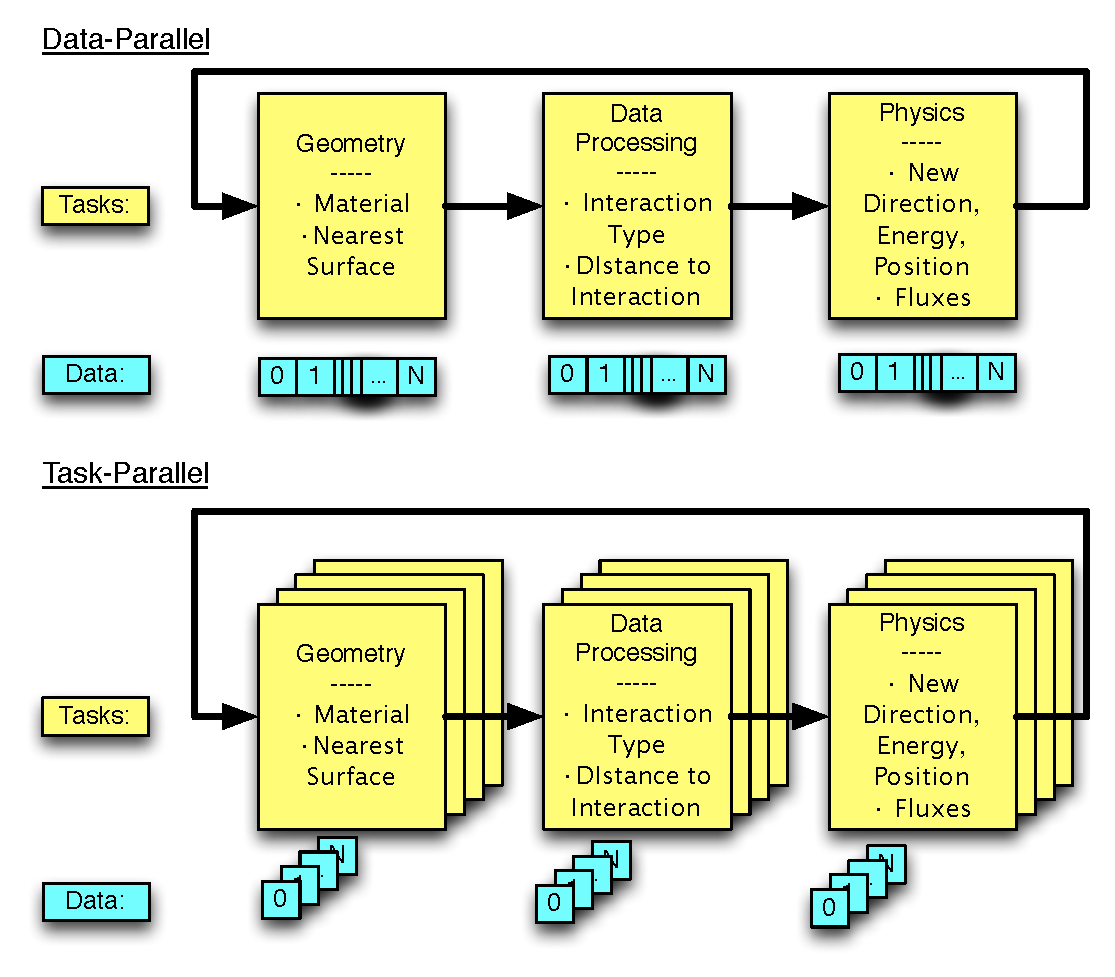
\includegraphics[width=\textwidth]{graphics/datavtask.pdf}
     \caption{A data-parallel neutron transport loop vs.\ a task-parallel transport loop for transporting N neutrons in parallel.  \label{datavtask} }
\end{figure}

In this paper, we start in Section~\ref{sec:background} discussing background information about GPUs and CPUs in the context of Monte Carlo neutral particle transport. Then, in Section~\ref{sec:features}, the current features of WARP are summarized while highlighting the newest developments.  The results of criticality calculations performed by WARP are compared against those from Serpent 2.1.24 \cite{jaakko,serpent} and MCNP 6.1 \cite{mcnp6}, two widely-used production-level Monte Carlo neutron transport codes.  This comparison is done to ensure the accuracy of WARP and to highlight performance differences.  The test case models used to conduct the comparisons are outlined in detail in Section~\ref{sec:tests}, then the run times, multiplication factors, and flux spectra calculated for the test cases are compared in detail in Section~\ref{sec:results}, after which a discussion is given summarizing comparisons and addressing any discrepancies shown in Section~\ref{sec:disc}.  Finally, conclusions about the initial development of WARP are drawn and future work is roughly outlined in Section~\ref{sec:concdev}. 
% The section references for the last two don't seem to be working right for me, but the refernces themselves should be right...


\section{Background}
\label{sec:background}
It seems that GPU cards would be perfect for running Monte Carlo neutron transport because they can run large numbers of concurrent threads.  
% It seems like you need another statement here. Like: ..."concurrent threads and there are large number of concurrent, independent tasks to be completed in MC" or soemthing like that.
However, this apparent perfect fit is complicated by how instructions are carried out on these threads.  
The concurrent thread number is based on the width of the processor's SIMD (single instruction multiple data) units.  SIMD is an execution model some processors use to lower the number of instructions needed per amount of computation done, which increases both power and computational efficiency \cite{simd_power}.  SIMD requires the same instructions to be carried out over every element in a concurrently-processed data vector.  From a thread standpoint, SIMD requires threads to execute the same instruction at one point in time.  If a set of threads does not execute the same instruction at the same time (the data they act on can be different), the GPU will serialize the operations.  In this case, the subset of threads executing the first instruction will all execute together, then the subset of threads executing the second instruction will all execute together after the first subset has completed. In the limit of each thread executing a different instruction, this becomes completely serial.  To most efficiently use SIMD by avoiding serialization, instruction regularity\footnote{DEFINITON} is required. Unfortunately, Monte Carlo typically breaks instruction regularity because of its conditional statements based on random numbers.  Therefore, if Monte Carlo algorithms are to be used on GPUs, they must be implemented in a manner that carefully takes into account the limitations of the GPU.

A further consideration is that the memory subsystems of GPUs also function in a SIMD-like way.  In order to use the full memory bandwidth of the device, more than one piece of data must be loaded and used per transaction, and the only way that multiple pieces of data can be loaded simultaneously is if they are adjacent in memory.  In other words, if a program requests a single piece of data at location $i$ and a piece at location $i+10$, these requests will be split into two separate transactions that each yield one data element.
%The original wording made it sound like these are two separate requests at different times ("and then"), whereas the sentence below makes it sound like the data are being requested at the same time. The apparent timing difference makes it seem like a false comparison. I _think_ this is the comparison that you want to make?
  Two data elements in two transactions produces an effective bandwidth of one element per transaction time. 
On the other hand, if the program requests data at $i$, $i+1$, $i+2$, and $i+3$, the entirety of the requested data can be retrieved in a single transaction.  Four data elements in a single transaction yields an effective memory bandwidth of four elements per transaction time, four times higher than the previous scenario.  Having a memory subsystem that handles requests in this way is not ideal for Monte Carlo methods, however.  In Monte Carlo data is accessed in a very random way because of the random nature of the simulation, and requested data is unlikely to be adjacent.  This means the full memory bandwidth of the GPU will not be used unless this problem is mitigated in some way.

Another challenge of using GPUs for Monte Carlo is GPUs have very high global memory latency compared to a CPU.  Memory latency is the number of clock cycles, or amount of time, it takes for a data request to be fulfilled.  As Table \ref{gpu_cpu_comp} shows, the GPU's global memory latency is about an order of magnitude higher than the CPU's \cite{cpu_latency,cuda}.  
GPUs try to eliminate the effect of large global latency by pipelining memory access.  Pipelining means threads that have received their data can execute as other threads are waiting for their data to load.  If many requests are known, the data can be continually loaded as threads start to execute their jobs.  The hope is that the jobs take longer than the memory loads, eventually all data arrives, and the later threads appear to have zero latency for their memory access.  This is why it is important for GPUs to have such a large number of concurrent threads.  It allows them to pipeline data access and minimize the impact of memory latency.

\begin{table}[h]
\centering
\caption[A comparison of an NVIDIA GPU and an Intel CPU]{NEEDS UPDATING.  A comparison of an NVIDIA GPU and an Intel CPU \cite{cent, cpu_latency, opteronperformance}.}
\label{gpu_cpu_comp}
\begin{tabular}{| l | r | r |}
\hline
Processor & Intel i7 & NVIDIA Tesla  \\
 &  (Westmere-EP) & C2075 (Fermi) \\
\hline
\hline
Processing Elements & 6 cores, 2 issue, & 14 cores, 2 issue, \\
& 4-way SIMD &  16-way SIMD  \\
\hline
Frequency & 3.46GHz &  1.15 GHz \\
\hline
Resident Strands / Threads (max) & 48 & 21,504 \\
\hline
SP GFLOPS & 166 & 1030 \\
\hline
Mem. Bandwidth &  32 GB/s & 144 GB/s \\
\hline
Global Latency & $\sim$50 clocks & 200-800 clocks  \\
\hline
FLOPS / byte & 5.2  & 7.2 \\
\hline
Register File & 6kB & 2MB \\
\hline
Local Storage / L1 Cache & 192 kB & 896 kB \\
\hline
L2 Cache & 1536 kB & 0.75 MB \\
\hline
L3 Cache & 12 MB & - \\
\hline
\end{tabular}
\end{table}

Another notable feature is that the GPU has a greater FLOPS/byte of memory bandwidth ratio than the CPU.  This implies that GPUs could be used to turn a compute-bound problem into a bandwidth-bound problem.  This may seem like a deficit, but the GPU has a higher maximum memory bandwidth, so even though a problem is bandwidth-bound on a GPU, it may still require less execution time than on a CPU.

The impetus for developing WARP was the research done by Martin and Brown in 1984 \cite{vector} for Monte Carlo and by Vuji\'{c} and Martin in 1991 \cite{vujic_vector} for the collision probability method.  In the 1984 paper, a method for mapping the Monte Carlo problem onto SIMD vector computers is described.  The essential idea in the 1984 paper was to bank the neutrons into vectors based on their required operation.  If a neutron was sampled to scatter, its data were placed into a buffer containing the data of other neutrons that have also been sampled to undergo scattering reactions.  If a neutron needs to do a surface crossing, it was placed into the surface crossing buffer, and so on.  Once a buffer became full, it was processed in a SIMD fashion by the vector computer.  Processing the neutron data further after the vector operation caused the buffers to contain non-uniform reactions, however, and a ``shuffle'' operation was done that actually moved data back into contiguous blocks based on the reaction type.  

This new approach was named ``event-based'' Monte Carlo, since the neutron events are tracked and processed as a group.  This was a very different way of performing a Monte Carlo simulation at the time.  Almost all computers were strictly serial, and SIMD lanes were only available in supercomputers.  Therefore, the pervasive method was the ``task-based" method in which neutrons are tracked for their entire lifetime in series.  Since GPUs are massively parallel and rely on SIMD, an event-based algorithm seemed to be the appropriate approach to GPU-accelerated neutron transport.  

Instead of trying to port an existing code to the GPU, the simplest way to accommodate requirements for efficient GPU execution was to write a new code from scratch.  This project ultimately resulted in WARP.  WARP uses an event-based algorithm, but with some important differences.  Vectorizing the Monte Carlo algorithm should allow for efficient GPU execution, but a paper by Zhang \cite{on_the_fly_remapping} also shows that by remapping data references, the thread divergence in GPU warps (groups of threads) can be minimized. Moving data is expensive, especially when the data set is large, so WARP uses a remapping vector of pointer/index pairs to direct GPU threads to the data they need to access.  The remapping vector is sorted  by reaction type after every transport iteration using a high-efficiency parallel radix sort (via the CUDPP library \cite{CUDPP}), which serves to keep the reaction types as contiguous as possible and removes completed histories from the transport cycle.  Sorting reduces the amount of divergence in GPU ``thread blocks,'' keeps the SIMD units as full as possible, and eliminates using memory bandwidth to check if a neutron in the batch has been terminated or not.  Using a remapping vector means the data access pattern is irregular, but this is mitigated by using large batch sizes where the GPU can effectively reduce the high cost of irregular global memory access.  The details about the existing algorithms used in WARP are discussed in \cite{algorithms} and will not be discussed in detail here.  New algorithmic changes since are discussed in Section \ref{sec:features}.

To use NVIDIA GPUs, parts of software must be written in a language that facilitates interaction with the GPU, and CUDA \cite{cuda}, a set of extensions for C/C++, was chosen.  CUDA was first released in 2006 as NVIDIA's proprietary GPU programming platform.  It makes minimal additions to C/C++, and any C programmer would be very comfortable programming in CUDA \cite{cuda}.  It was chosen over OpenCL, the open source GPU programming platform, because of CUDA's greater feature support, stability, ease of programming, wider community usage, and ability to use new, cutting-edge features in NVIDIA GPUs that OpenCL does not have.


%%%%%%%%%%%%%%%%%%%
%%%%%%%%%%%%%%%%%%%
%%%%%%%%%%%%%%%%%%%
\section{Features of WARP}
\label{sec:features}

WARP has only existed since 2013, and is not as fully-featured as more mature Monte Carlo codes.  However, it has the functionality necessary to compare its performance against Serpent 2.1.24 and MCNP 6.1; this section outlines the current set of features available in WARP.  WARP is mainly written in C/C++ and is compiled to a shared library.  With the shared library compiled, a user must write a \texttt{main()} function that calls the library routines and directs program flow.  Pythonic wrapping of the shared library is done via SWIG \cite{swig}, which automatically wraps compiled languages like C/C++ in high-level scripting languages.  With the C++ classes exposed in Python, the \texttt{main()} function can be replaced with a Python script, eliminating the need to recompile a main function and link it to the WARP library when different geometries or different run parameters are desired.  This is why WARP is termed a ``framework'' rather than a ``program.''  Of course, there is flexibility in the setup as well, and a user could write a main function that could handle all conceivable input cases and would never have to recompile the \texttt{main()} function.  
% The way this is written now, it's not clear why it needs to be recompiled as is and what would need to be different to avoid this.

The Python wrapping approach deviates from the standard flat text input file structure that many Monte Carlo codes use.  Flat text input/output relies on keywords  and/or regular formatting, which adds a layer between simulation and analysis.  Using Python to directly access the classes and their data removes this layer and allows a user to build complex, custom applications as desired.  With Python, the results of a calculation are also resident in a Python session and are therefore easily available to the user for plotting with scripts or processing with other analysis tools.  To process data in the same way from a text file output, the output would need to be parsed with a user-written function or processed by hand, which is time-consuming and can lead to human error.

\subsection{Physics}

Only neutrons are transported by WARP.  Any other particles are not considered in any way.  Cross section data compiled by the United States is distributed by the Department of Energy in \emph{ENDF} files.  ENDF stands for ``evaluated nuclear data file'' and can contain data for nuclear decay, photons, atomic relaxation, fission yields, thermal neutron scattering, and charged particle reactions as well as neutron reactions.   WARP loads ACE-formatted nuclear data libraries via the ``ace'' module in PyNE (Python for Nuclear Engineering) \cite{pyne}.  This module has been separated from PyNE and included as a standalone Python module with WARP.  Including it as a separate module with WARP means the entire PyNE package does not need to be installed in order to compile and run WARP.  ACE stands for ``a compact ENDF'' and strips out much of the extra information unnecessary for neutron transport and formats the data into the specified tabulation \cite{endfnums}.  Since many Monte Carlo codes read ACE-formatted data rather than the original ENDF file, WARP can eliminate one potential cause for discrepancies by loading the same data as other codes.  The cross section data are then reformatted to use a unionized energy grid via NumPy \cite{numpy}; the reformatted data are then passed to the C++ routines via the Python C API.

In its current state, WARP does not use S($\alpha,\beta$) thermal scattering tables or unresolved resonance parameters.  It only uses the free-gas approximation to account for the motion of material nuclei.  The free-gas approximation treats the target as part of a gas at a certain temperature and does not consider other modes of energy transfer that rise from inter- and intra-molecular phenomena.  Thermal scattering and unresolved resonance data improve the physical fidelity of the simulation, but these features were turned off in production codes so that WARP could be directly compared to them. 

WARP currently has an incomplete set of the ENDF sampling laws implemented: laws 3 (level scattering), 4 (continuous tabular distribution), 7 (simple Maxwell fission spectrum), 9 (evaporation spectrum), 11 (energy-dependent Watt spectrum), 44 (Kalbach-87 formalism), 61 (LAW=44 but tabular angular distribution), and 66 (N-body phase space distribution) \cite{MCNP}.  These laws cover all the reactions present in the test problems presented here and most nuclides in the ENDF/B-VII.1 cross section data set, but some nuclei may have interactions that require the remaining neutron sampling laws: 1 (tabular equiprobable energy bins), 5 (general evaporation spectrum), 22 (tabular linear functions), 24 (UK law 6), and 67 (laboratory angle-energy law).  Problems containing any such nuclides cannot be simulated with the current version of WARP, but could be added later.  These unincluded laws are not nearly as common as the ones currently included in WARP, and excluding them at this point should not greatly impact the ability to benchmark WARP's performance and accuracy.

WARP only has collision estimators implemented for both flux and multiplication factor estimation.  The relative error of these estimations are calculated, but any additional convergence estimation beyond relative error has not been implemented.  Variance reduction is not implemented in WARP.  Neutrons have statistical weight in WARP, and currently the only reactions that adjust neutron weight are multiplicity reactions, like (n,2n), where the neutron weight is multiplied by the exiting neutron number in a manner similar to OpenMC \cite{openmc}.  This means that new neutron histories do not have to be created mid-batch in criticality calculations, and makes program flow simpler.  Analog capture was turned on in Serpent and MCNP in all simulations considered to ensure a fair comparison of the results.  

\subsection{Geometry}

The geometry representation in WARP is handled by the NVIDIA OptiX ray tracing framework \cite{optix}.  OptiX provides good performance on the GPU, but imposes some limitations on the how geometries must be input.  For the current algorithm used, the geometrical limitations are:

\begin{enumerate}
\item Cells are the basic building blocks of a model, not surfaces.
\item All cells must be finite, closed, and non-overlapping.
\item Implicit nesting determines what material exists inside of a cell.  In other words, since cells are defined directly, the material of cell A is only that space where cell A is the lowest nested cell.  If cell B is within cell A, the entire space within cell B is excluded from cell A simply because cell B resides within cell A.  It does not need to be excluded explicitly.
\item The only cell types available are spheres, cylinders, right rectangular prisms, and right hexagonal prisms.
\item Only translational transforms have been implemented.
\item Vacuum (i.e.\ infinitely absorbing) and specular reflection  (i.e.\ mirror) boundary conditions are available.
\end{enumerate}

An improved tracking routine, which determines which cell a neutron resides in based on its spatial coordinates, has been implemented in WARP since the last publication \cite{algorithms}.  Previously, a ray was traced from the neutron position to the outer cell, and a list of cell numbers was stored, in order, for each intersection.  The double entries were removed as the list was written, which, at the end of the trace, yielded a list of cells the neutron was nested in.  This resulted in very poor performance in deeply-nested cases due to this list becoming large.  For example, WARP had very significant performance decreases in the Jezebel spherical criticality test (discussed later) if the sphere was segmented into many spherical shells.  Doing this caused WARP to store a long list of surface numbers and made the simulation very slow.  
WARP now uses ``cell sense'' to reduce the memory impact of determining in which cell/material a neutron resides.  ``Surface sense'' is a basic feature of many computational solid geometry (CSG) systems, and is simply the sign of the remainder left after evaluating a set of coordinates in a surface equation. ``Cell sense'' is like surface sense in that it is positive if a neutron is outside a cell and is negative if a neutron is inside the cell.  Cell sense can be calculated by taking the product of the surface senses of the cell's constituent planes.  In the new and improved tracking routine, the cell sense (which is either 1 or -1) is calculated and summed as the query ray traverses the geometry.  When the sum becomes negative, the last intersected surface is the cell in which the neutron is located.   Figure \ref{whereami} shows an illustration of the new geometry query algorithm.  Using the new surface sense traversal method results in high performance even in the previously mentioned segmented Jezebel case.

\begin{figure}[h!]
\centering
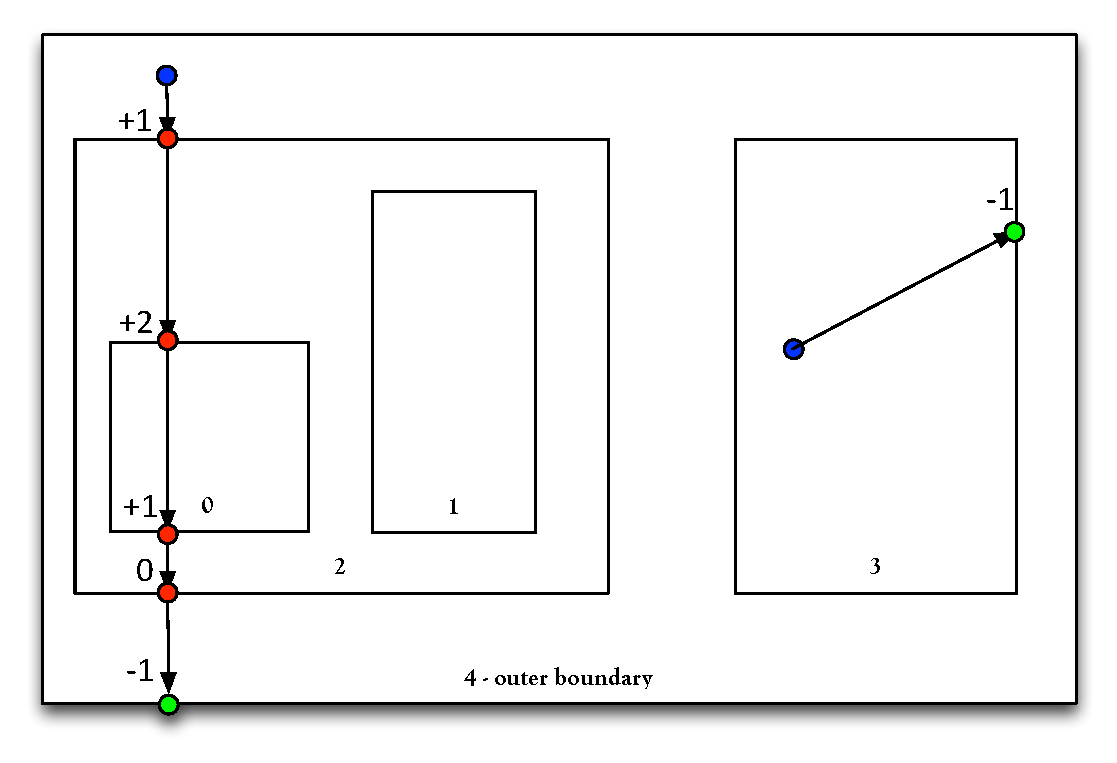
\includegraphics[width=0.75\textwidth]{graphics/whereami-new.pdf}
\caption{The improved geometry query algorithm showing how the cell number is calculated through ray tracing.  A ray is iteratively drawn from the neutron starting position to the outer cell, and the surface normal values are summed along the way.  When the sum reaches -1, the cell in which the neutron resides has been found and the trace stops. \label{whereami} }
\end{figure}

 When the cumulative sense becomes negative, the containing cell has been intersected and tracing can stop.  This approach can be used because all bodies must be closed.  This scheme takes advantage of the acceleration structure in OptiX while still using the simplicity of combinatorial solid geometry.  It essentially is the same scheme as MCNP/Serpent, except that the acceleration structures allow surfaces that are part of cells that are far away to be skipped.  Also, compared to the past scheme of storing a list of doubles, this method requires a single integer to be stored and operated on instead of a potentially large and slow list. 

Since OptiX allows variables to be attached to individual geometrical objects, this feature has been exploited in order to create an efficient general tally routine.  After the geometry has been input and desired tallies have been specified, WARP creates an array of tally data structures and attaches the tally index directly to each geometrical object that the tally is associated with.  When OptiX is called to calculate the nearest intersection points and determine which cell a neutron is in, it also reports back the index of the tally (if any) that should be scored at a collision.  This way, the high performance of the OptiX library is leveraged to perform the hash between cell number and tally index, and a separate search does not have to be performed.  The material index is returned by OptiX in an identical way.


%%%%%%%%%%%%%%%%%%%
%%%%%%%%%%%%%%%%%%%
%%%%%%%%%%%%%%%%%%%
\newpage
\section{Tests}
\label{sec:tests}

A small set of CPU and GPU platforms were chosen for use in testing WARP.  These platforms were chosen simply because they were easily accessible from UC Berkeley.  For the CPU platforms, a single cluster node of both Berkelium (Bk), the departmental cluster, and Savio2, the shared campus high performance computing cluster, were used.  For the GPU platforms, a consumer-level graphics card and two compute-specific cards were used.  Descriptions of each piece of hardware can be found in Table~\ref{platform_table}. For the GPUs, the costs include the retail price of a minimal host computer with at least as much memory as the card ({\raise.17ex\hbox{$\scriptstyle\sim$}}\$400).
  

\begin{table}[h]
\centering
\caption{Platforms used in the benchmark cases and their specifications.}
\label{platform_table}
\small
\begin{tabular}{| l | r | r | r | r |}
\hline
\multirow{2}{*}{Platform} &  Cost   &Total Processor  & Local       & Memory     \\
                                       & (USD)  & Power (Watts) & Memory  & Frequency \\
\hline
Bk PSSC PowerWulf Blade       &    9,310   & 460 &  96 GB        &  1.6 GHz                    \\
\hline
Savio2 Lenovo NeXtScale nx360 M5       &   6,770    &  210  &  64 GB        & 2.133  GHz                    \\
\hline
NVIDIA Tesla K20         &    3,325     & 225 &  4.8  GB      &  2.6 GHz                  \\
\hline
NVIDIA Titan Black       &    1,521   & 250 &  6.14 GB        & 3.5 GHz              \\
\hline
NVIDIA Tesla K80       &    5,000    & 300 &  12 GB        &  2.505 GHz              \\
\hline
\hline
\hline
\multirow{2}{*}{Platform}  &  \multicolumn{2}{r|}{Physical }     & Processor  & Maximum \\
                                        & \multicolumn{2}{r|}{Processors}  & Frequency  & Threads \\
\hline
Bk PSSC PowerWulf Blade       &   \multicolumn{2}{r|}{4x AMD Opteron 6172 }  &  2.1 GHz     &  48           \\
\hline
Savio2 Lenovo NeXtScale nx360 M5   &   \multicolumn{2}{r|}{ }  &  2.3 GHz     &  24           \\
\hline
NVIDIA Tesla K20         &       \multicolumn{2}{r|}{13}   &  705.5 MHz     &  $2^{32}-1$           \\
\hline
NVIDIA Titan Black       &      \multicolumn{2}{r|}{ 15 }  &  1071.5 MHz     & $2^{32}-1$           \\
\hline
NVIDIA Tesla K80      &      \multicolumn{2}{r|}{ 13 }  &  823.5 MHz     & $2^{32}-1$           \\
\hline

\end{tabular}
\end{table}

All tests use ENDF/B-VII cross sections that are distributed with the Serpent 1.1.7 release from RSICC (Radiation Safety Information Computational Center), which regulates the licensing and distribution of the MCNP and ENDF data worldwide, and also distributes Serpent 1.1.7.  These cross sections contain fewer energy grid points than the ENDF/B-VII.1 cross sections that are distributed with the MCNP 6.1 release from RSICC.  Since the Serpent 1.1.7 data require less storage space, using them allows more isotopes to be used by WARP.


%%%%%%%%%%%%%%%%%%%
\newpage
\subsection{Test 1 - ``Jezebel'' Bare Pu Sphere}

The ``Jezebel'' criticality test is a bare plutonium/gallium sphere with vacuum boundary conditions, which can be seen in Figure~\ref{jezebel_geom_pic}.  The fission neutron rate from $^{239}$Pu is balanced by the leakage rate from the 6.6595 cm radius to give a $k_\mathrm{eff}$ of approximately 1.  Since this system is so leaky, producing results consistent with MCNP and Serpent ensures that the boundary conditions are correctly being enforced.  The Jezebel test is a standard test used to validate neutron transport codes and is described in the International Handbook of Evaluated Criticality Safety Test Experiments under the name ``Pu-MET-FAST-001'' \cite{bench_handbook}.  The geometry and materials are outlined in Table \ref{jezebel_geom}.  All cross sections used were processed at 273.5 K.

\begin{figure}[h!] 
  \centering
    
\includegraphics[width=0.4\textwidth]{graphics/jezebel-xy.png}
     \caption{ Horizontal slice of the geometry of the ``Jezebel'' test case.  Colors represent cell numbers and black represents space outside the outermost boundary. \label{jezebel_geom_pic} }
\end{figure}

\begin{table}[h]
\centering
\caption{Geometry and materials used in the ``Jezebel'' test case.}
\label{jezebel_geom}
\begin{tabular}{| l | c  c | c |}
\hline
Cells & Isotopes & (Atm. \%)& Density \\
\hline
\multirow{3}{*}{1 sphere, r=6.6595 cm }  &  $^{239}$Pu (0.7381)    &    $^{240}$Pu (0.1942)     &  \multirow{3}{*}{15.73 g/cm$^3$} \\
                                         &  $^{241}$Pu (0.0299)    &     $^{242}$Pu (0.0038)    &   \\
                                         &  $^{69}$Ga  (0.0203)    &     $^{71}$Ga  (0.0135)    &   \\
\hline
\end{tabular}
\end{table}

%%%%%%%%%%%%%%%%%%%
\newpage
\subsection{Test 2 - Homogenized Fuel Block}

The homogenized block criticality test is a bare cube with vacuum boundary conditions as seen in Figure~\ref{homfuel_geom_pic}.  This test keeps the same boundary condition, temperature, and number of cells as test 1, but is larger (reducing leakage), contains light isotopes (which readily produce thermal neutrons), and introduces new isotopes.  Introducing new isotopes into the simulation is significant in that new isotopes may use any of the various sampling laws outlined earlier.  Comparing spectra from calculations containing many different isotopes simply shows that WARP can handle sampling the laws correctly.  The geometry and materials are outlined in Table \ref{homfuel_geom}.  All cross sections used were processed at 273.5 K.

\begin{figure}[h!] 
  \centering
    
\includegraphics[width=0.4\textwidth]{graphics/homfuel-xy.png}
     \caption{ Horizontal slice of the geometry of the homogenized fuel block test case.  Colors represent cell numbers and black represents space outside the outermost boundary. \label{homfuel_geom_pic} }
\end{figure}

\begin{table}[h]
\centering
\caption{Geometry and materials used in the homogenized fuel block test case.}
\label{homfuel_geom}
\begin{tabular}{| l | c  c | c |}
\hline
Cells & Isotopes & (Atm. \%)& Density \\
\hline
\multirow{5}{*}{1 cube, 100x100x50 cm }            &   $^{238}$U   (0.90)   &  $^{235}$U   (0.10)   &  \multirow{5}{*}{5.50 g/cm$^3$} \\
                                                   &   $^{16}$O    (3.00)   &  $^{2}$H     (2.0)    &  \\
                                                   &   $^{90}$Zr   (0.5145) &  $^{91}$Zr   (0.1122) &  \\
                                                   &   $^{92}$Zr   (0.1715) &  $^{94}$Zr   (0.1738) &  \\
                                                   &   $^{96}$Zr   (0.0280) &                       &  \\
\hline
\end{tabular}
\end{table}



%%%%%%%%%%%%%%%%%%%
\newpage
\subsection{Test 3 - Zr-Clad UO$_2$ Pin in Heavy Water}

This criticality test, shown in Figure~\ref{pincell_geom_pic}, consists of a UO$_2$ cylinder clad in zirconium surrounded by a large block of light water.  This test increases complexity by having three materials, each with multiple isotopes, and three cells.  The water block has vacuum boundary conditions.  Its dimensions are relatively large and the absorption is low, so the mean neutron lifetime should be large.  This test serves to demonstrate that all the processing routines work simultaneously,
% what does that mean?
 the effect of introducing more than one cell, and the effect of long-lived neutrons.  The geometry and materials are outlined in Table \ref{uo2_pincell_geom}.  All cross sections used were also processed at 273.5 K.

\begin{figure}[h!] 
  \centering
    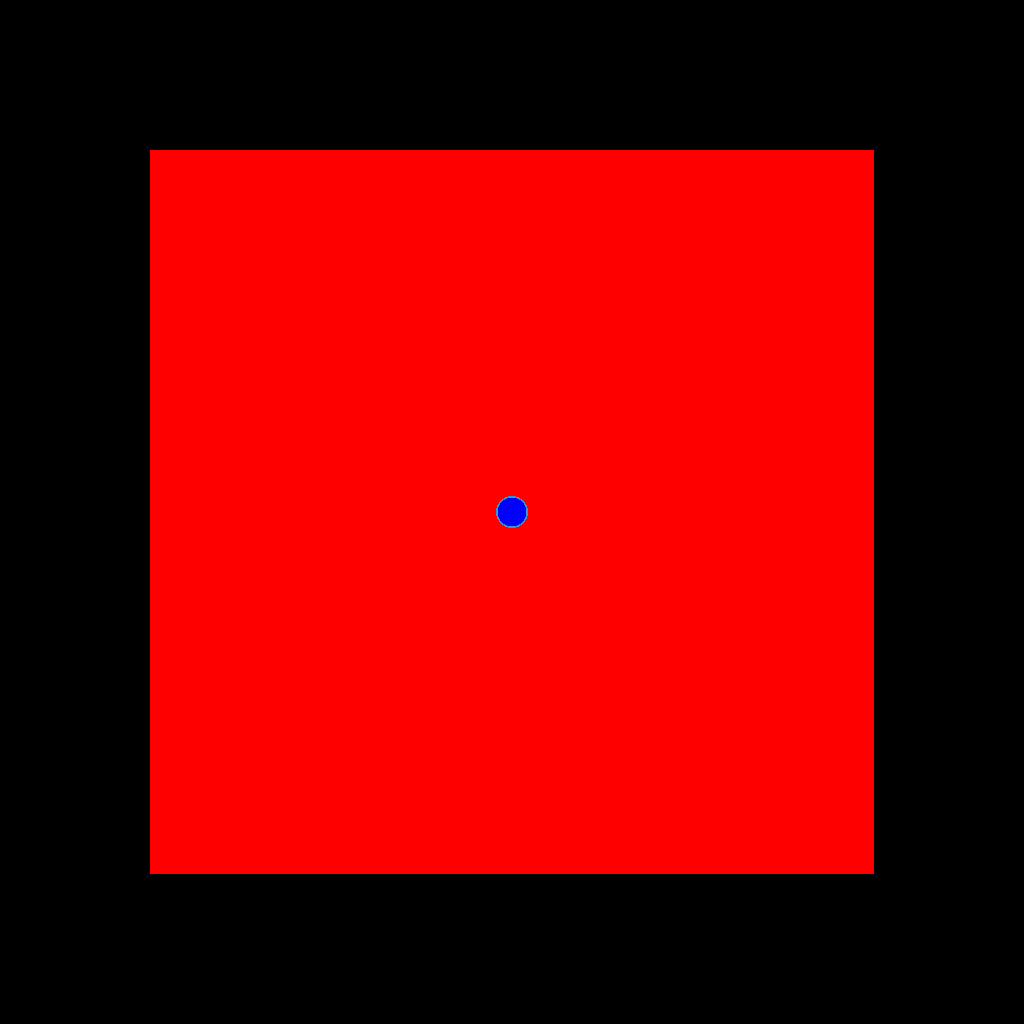
\includegraphics[width=0.4\textwidth]{graphics/pincell-xy.png}
     \caption{  Horizontal slice of the geometry of the Zr-clad UO$_2$ pin in heavy water test case.  Colors represent cell numbers and black represents space outside the outermost boundary. \label{pincell_geom_pic} }
\end{figure}

\begin{table}[h]
\centering
\caption{Geometry and materials used in the single UO$_2$ pin in D$_2$O test case.}
\label{uo2_pincell_geom}
\begin{tabular}{| l | c  c | c |}
\hline
Cells & Isotopes & (Atm. \%)& Densities \\
\hline
\multirow{2}{*}{1 cylinder, r=2.0 cm z=$\pm$20 }  &   $^{238}$U   (0.90) &  $^{235}$U   (0.10) &  \multirow{2}{*}{10.97 g/cm$^3$} \\
                                                                              &   $^{16}$O    (2.00)  &                              &  \\
\hline
\multirow{3}{*}{1 cylinder, r=2.2 cm z=$\pm$20.2}  &   $^{90}$Zr   (0.5145) &  $^{91}$Zr   (0.1122)&  \multirow{3}{*}{6.52 g/cm$^3$} \\
                                                   &   $^{92}$Zr   (0.1715) &  $^{94}$Zr   (0.1738)& \\
                                                   &   $^{96}$Zr   (0.0280) &                      & \\
\hline
\multirow{1}{*}{1 box, 50x50x50 cm }  &    $^{2}$H   (2.0) & $^{16}$O   (1.0) &   \multirow{1}{*}{1.11 g/cm$^3$} \\
\hline
\end{tabular}
\end{table}

% Everywhere, I'd consider bolding table headings so they stick out a bit more.


%%%%%%%%%%%%%%%%%%%
\newpage
\subsection{Test 4 - Homogenized Fuel Pebble in FLiBe}

This criticality test consists of a single sphere of homogenized UO$_2$ and C surrounded by molten FLiBe (Li$_2$BeF$_4$) salt, shown in Figure~\ref{flibe_geom_pic}.  The outer cell is a right hexagonal prism with specular reflective boundary conditions.  This test uses two temperatures simultaneously and tests the reflective boundary condition setting.  The geometry and materials are outlined in Table \ref{pebble_geom}, where ``r'' shown for the hex prism is the length of the apothem.  The FLiBe cross sections used were processed at 900 K and the pebble cross sections at 1200 K.

\begin{figure}[h!] 
  \centering
    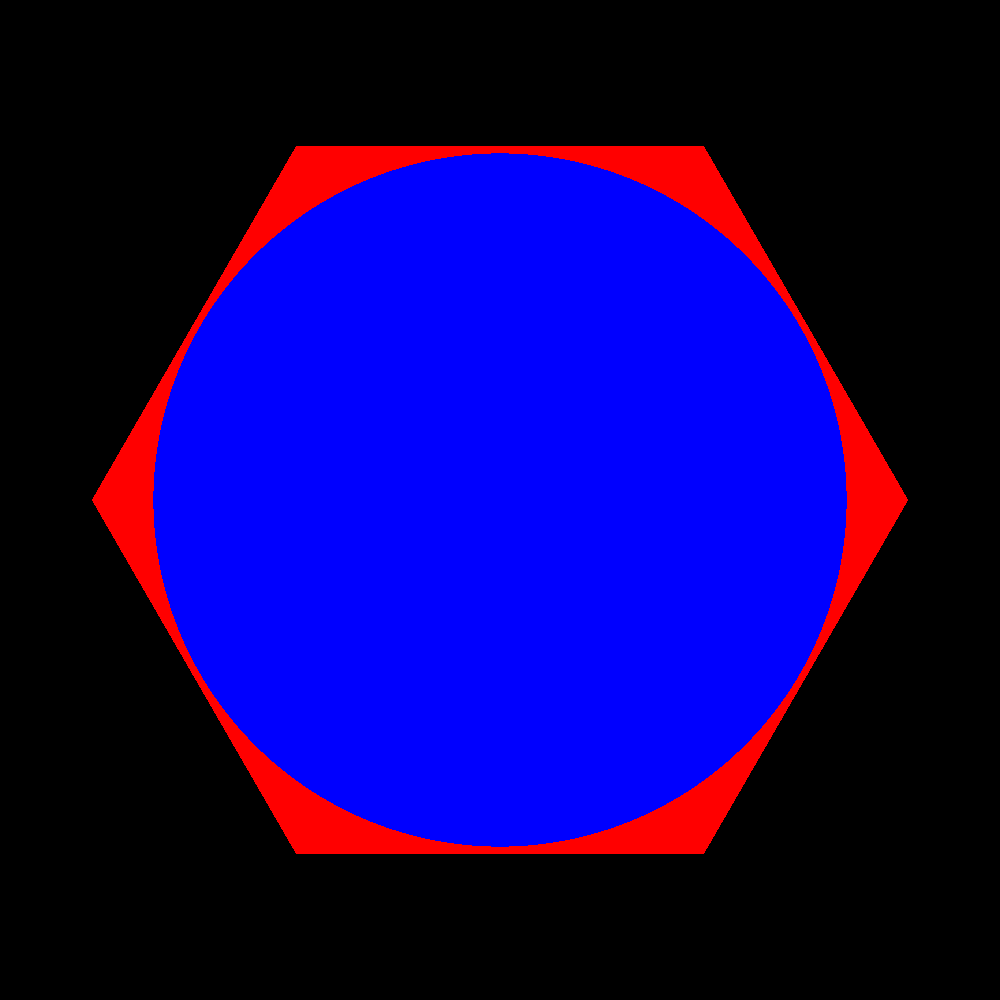
\includegraphics[width=0.4\textwidth]{graphics/flibe-xy.png}
     \caption{ Horizontal slice of the geometry of the homogenized fuel pebble in FLiBe test case.  Colors represent cell numbers and black represents space outside the outermost boundary. \label{flibe_geom_pic} }
\end{figure}

\begin{table}[h]
\centering
\caption{Geometry and materials used in the pebble in molten FLiBe test case.}
\label{pebble_geom}
\begin{tabular}{| l | c  c | c |}
\hline
Cells & Isotopes & (Atm.  \%)& Densities \\
\hline
\multirow{3}{*}{1 sphere, r=5.0 cm }  &   $^{238}$U   (0.90) &  $^{235}$U   (0.10) &  \multirow{3}{*}{8.75 g/cm$^3$} \\
                                      &   $^{16}$O    (2.00) &  $^{12}$C    (1.978) &  \\
                                      &   $^{13}$C    (0.022)&                     &  \\
\hline
\multirow{2}{*}{1 right hex prism, r=5.1 cm }  &   $^{6}$Li  (0.15) &  $^{7}$Li  (1.85)&  \multirow{2}{*}{1.94 g/cm$^3$} \\
                                               &  $^{9}$Be  (1.00) & $^{19}$F  (4.00) &  \\
\hline
\end{tabular}
\end{table}

%%%%%%%%%%%%%%%%%%%
\newpage
\subsection{Test 5 - Stainless Steel Clad Metallic Uranium Pin in Liquid Sodium}

The criticality test in Figure~\ref{sodiumpin_geom_pic} consists of a single cylinder of metallic uranium surrounded by molten sodium.  The outer cell is a right hexagonal prism with specular reflective boundary conditions.  This test serves to benchmark a fast system with a coolant as well as introduce more and different isotopes.  The geometry and materials are outlined in Table \ref{sodium_geom}.  The fuel and clad cross sections used were processed at 900 K, and the sodium coolant cross sections were processed at 600 K.  In order to keep the specification tenable, only the major components of 316 stainless steel were included in the clad material. 

\begin{figure}[h!] 
  \centering
    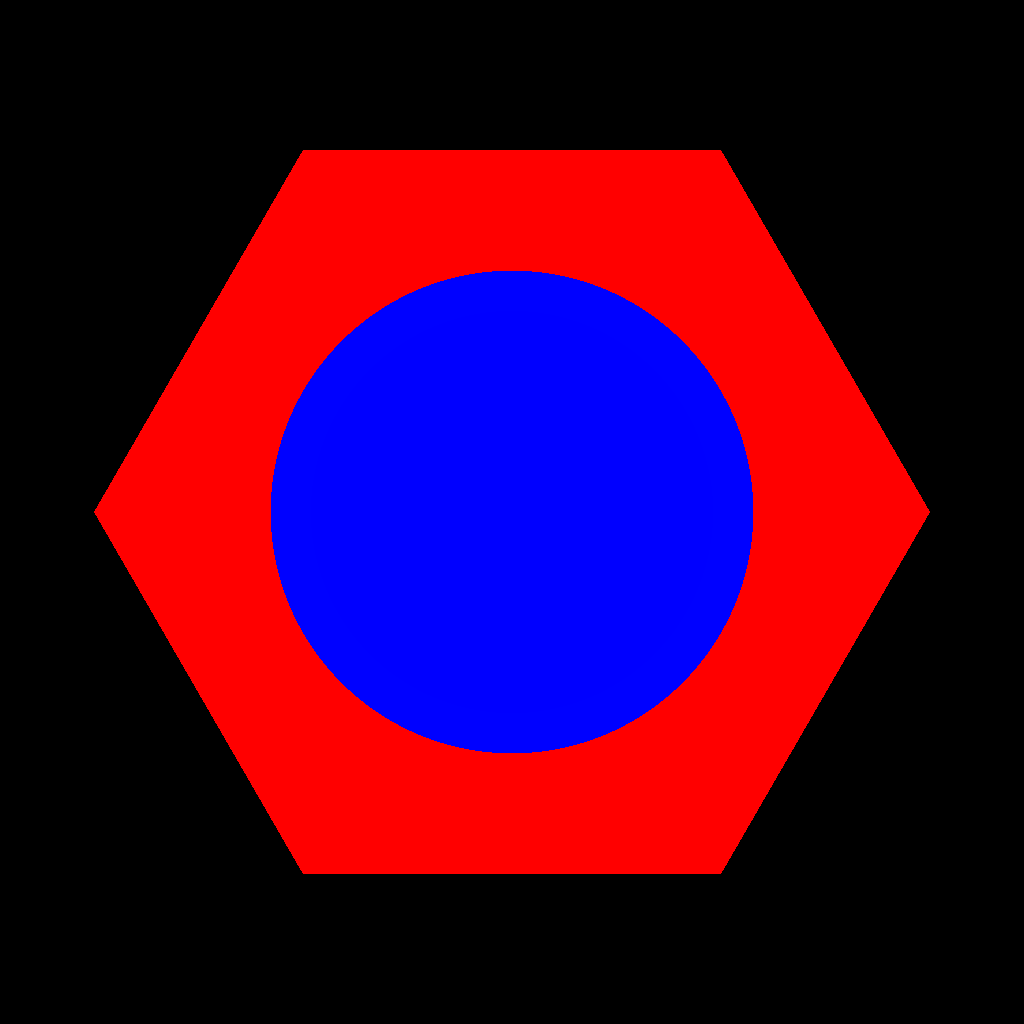
\includegraphics[width=0.4\textwidth]{graphics/sodiumpin-xy.png}
     \caption{ Horizontal slice of the geometry of the stainless steel clad metallic uranium pin in liquid sodium test case.  Colors represent cell numbers and black represents space outside the outermost boundary. \label{sodiumpin_geom_pic} }
\end{figure}

\begin{table}[h]
\centering
\caption{Geometry and materials used in the 316 stainless steel clad metallic uranium single pin test case.}
\label{sodium_geom}
\begin{tabular}{| l | c  c  | c |}
\hline
Cells & Isotopes & (Atm. \%)     & Densities \\
\hline
\multirow{1}{*}{1 cylinder, r=1.0 cm }   &  $^{238}$U   (0.90)   & $^{235}$U   (0.10)   &    \multirow{1}{*}{19.1 g/cm$^3$} \\
\hline
\multirow{6}{*}{1 cylinder, r=1.2 cm }   &  $^{54}$Fe  (0.0435) & $^{56}$Fe  (0.6879)  &   \multirow{6}{*}{7.99 g/cm$^3$} \\
                                         &  $^{57}$Fe  (0.0165) & $^{58}$Fe  (0.0021)  &   \\
                                         &  $^{50}$Cr  (0.0065) & $^{52}$Cr  (0.1257)  &   \\
                                         &  $^{53}$Cr  (0.0143) & $^{54}$Cr  (0.0035)  &   \\
                                         &  $^{58}$Ni  (0.0681) & $^{60}$Ni  (0.0262)  &   \\
                                         &  $^{62}$Ni  (0.0036) &  $^{64}$Ni  (0.0009) &   \\
\hline
1 right hex prism, r=1.8 cm              &  $^{23}$Na   (1.00)  &                      &    0.927 g/cm$^3$ \\
\hline
\end{tabular}
\end{table}


%%%%%%%%%%%%%%%%%%%
\newpage
\subsection{Test 6 - Zr-Clad Hexagonal UO$_2$ Pin Cell Lattice in Light Water}

This criticality test consists of 631 Zr-clad UO$_2$ cylinders laid out in a hexagonal lattice surrounded by light water, as shown in Figure~\ref{hex_geom_pic}.  The material compositions, densities, and cylinder dimensions are similar to the pin cell test case, but, since this test has two orders of magnitude more objects, it serves to highlight the effect of introducing many geometric objects into the problem and further validates that the geometry processing routines work correctly.  The lattice is in the x-y plane, has a pitch to diameter ratio of 1.164, and has 15 elements on a side.  The geometry and materials are outlined in Table \ref{hex_geom}.  All cross sections used were processed at 273.5 K.

\begin{figure}[h!] 
  \centering
    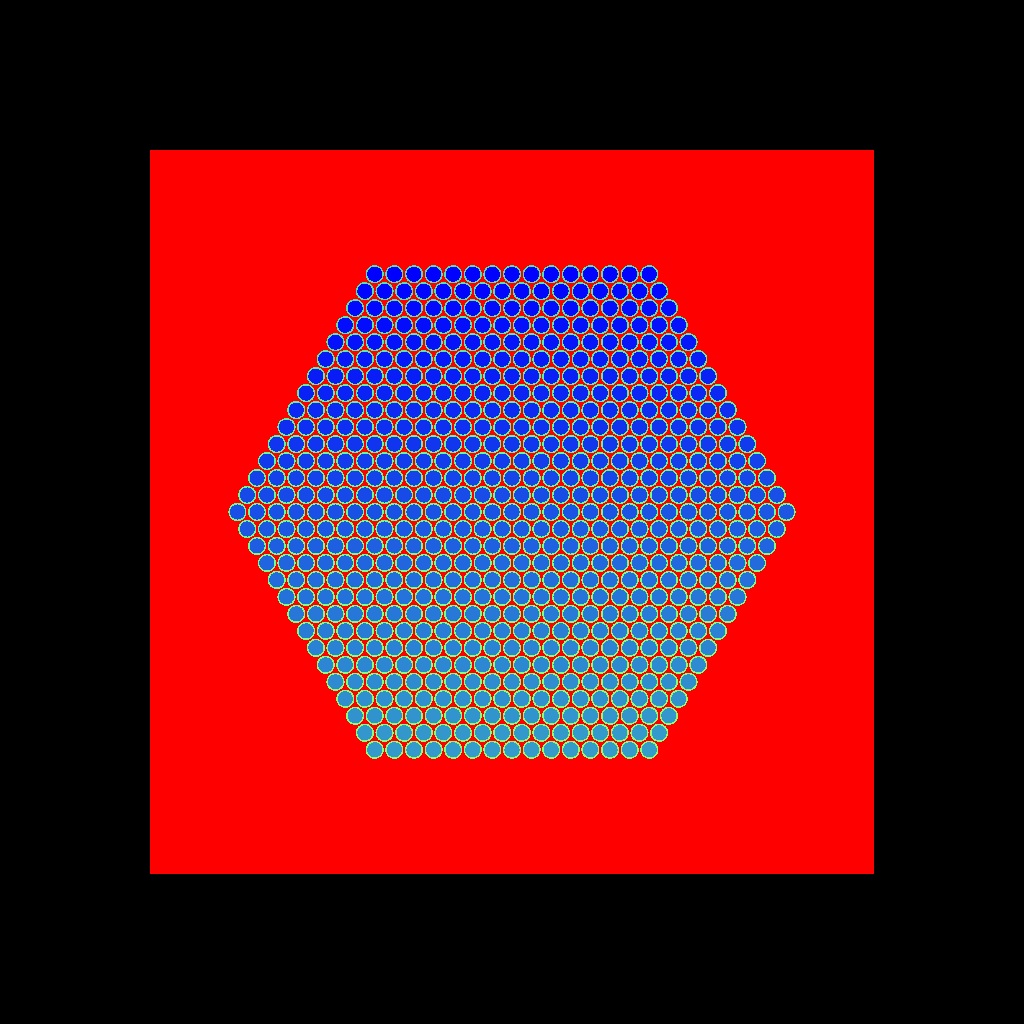
\includegraphics[width=0.4\textwidth]{graphics/assembly-lw-xy.png}
     \caption{ Horizontal slice of the geometry of the Zr-clad hexagonal UO$_2$ pin cell lattice in light water test case.  Colors represent cell numbers and black represents space outside the outermost boundary. \label{hex_geom_pic} }
\end{figure}

\begin{table}[h]
\centering
\caption{Geometry and materials used in the Zr-clad UO$_2$ pin hexagonal lattice in light water test case.}
\label{hex_geom}
\begin{tabular}{| l | c  c | c |}
\hline
Cells & Isotopes & (Atm. \%) & Densities \\
\hline
\multirow{2}{*}{631 cylinders, r= 1.0 cm }  &   $^{238}$U   (0.90)   &    $^{235}$U   (0.10)  &  \multirow{2}{*}{10.97 g/cm$^3$} \\
                                           &   $^{16}$O    (2.00)   &                        &  \\
\hline
\multirow{3}{*}{631 cylinders, r= 1.2 cm }  &   $^{90}$Zr   (0.5145) &    $^{91}$Zr   (0.1122)&  \multirow{3}{*}{6.52 g/cm$^3$} \\
                                           &   $^{92}$Zr   (0.1715) &    $^{94}$Zr   (0.1738)& \\
                                           &   $^{96}$Zr   (0.0280) &                        & \\
\hline
\multirow{1}{*}{1 box, r= 1.0 cm }         &   $^{1}$H     (2.0)    &   $^{16}$O  (1.0) & \multirow{1}{*}{1 g/cm$^3$} \\
\hline
\end{tabular}
\end{table}




%%%%%%%%%%%%%%%%%%%
%%%%%%%%%%%%%%%%%%%
%%%%%%%%%%%%%%%%%%%
\section{Results}
\label{sec:results}
 

The accuracy of the WARP calculations were measured by comparing the multiplication factors and neutron spectra of the aforementioned geometries against those calculated by Serpent 2.1.24 and MCNP 6.1.  The multiplication factor differences shown in this section are reported in ``per cent mille'' (PCM), which is a thousandth of a percent, or $10^{-5}$.  This is a standard way of reporting differences in the multiplication factor, as any small change in it can cause a significant change in system behavior.  The flux spectra are normalized per fission neutron and per unit lethargy.   ``Lethargy'' means the logarithm of the neutron energy, $\ln(E_0/E)$, where $E_0$ is the highest energy possible in a system and $E$ is another energy \cite{duderstadt}.  Normalizing the flux per unit lethargy in conjunction with plotting on a logarithmic scale yields a plot where the area under the curve gives the fraction of neutrons flux within the bounding energy range. 

The performance of WARP is measured by comparing the runtimes of the WARP simulations against those of the production codes.  The runtimes do not include the time it takes to load and process cross sections before the simulations.  In other words, it is only the time it takes to complete all transport cycles.  The difference in runtimes are reported in speedup factors ($t/t_\mathrm{WARP}$).  The times reported are either for simulations performed on a single card or a single node.  This was done to compare the platforms fairly.  Resources are shared at the single card/node level, and therefore increasing process and/or thread count does not necessarily scale linearly as resource contention increases.  It can be optimistically assumed that scaling occurs linearly above this level if little inter-card/node communication is needed, and therefore speedup ratios comparing single-node/card performance should be equivalent to multi-node/card performance.

The benchmark cases were run with $6.5\times10^6$ neutrons per criticality batch with 20 initial batches discarded and 40 batches with statistics accumulated (60 batches total).  From the scaling results shown next in this section, the neutron processing rate of the GPU cards all saturated near this number of neutrons per batch.  The CPU codes were run with identical batch parameters.  The CPU cases were run with the optimal number of MPI processes and threads per process for the specific node to fairly measure the performance of the unit as a whole.  Since the PowerWulf PSSC node contains 4 processors that each contain 2 non-uniform memory access (NUMA) nodes, the most efficient configuration for running the CPU codes was to use 8 MPI processes (one for each NUMA node), which each ran 6 threads for the 6 cores in each NUMA node.  The Lenovo Savio2 runs were done in a similar way, but with 4 MPI processes that each ran 6 threads.  The MCNP runs were launched with one additional MPI process since the master process does not perform any neutron tracking in MCNP.  All codes were set to not use thermal scattering or unresolved resonance tables and to use analog capture only.

\subsection{Scaling}

Larger neutron datasets allow the GPU to schedule threads better, but the size of the dataset is limited by the available on-card memory.  Cross sections are also stored on-card and compete with the neutrons for space in memory.  It is of interest to know where performance saturates so a user can choose to run the number of neutrons per cycle that gives the best performance.  Figure \ref{scaling} shows the neutron processing rate of WARP compared to the neutron dataset size.

%KR - can the legend of this plot be fixed to capitalize the k's in K20 and K80? the plotting script has the correct capitalizations but the scaling plot here doesn't.
\begin{figure}[h!]
\centering
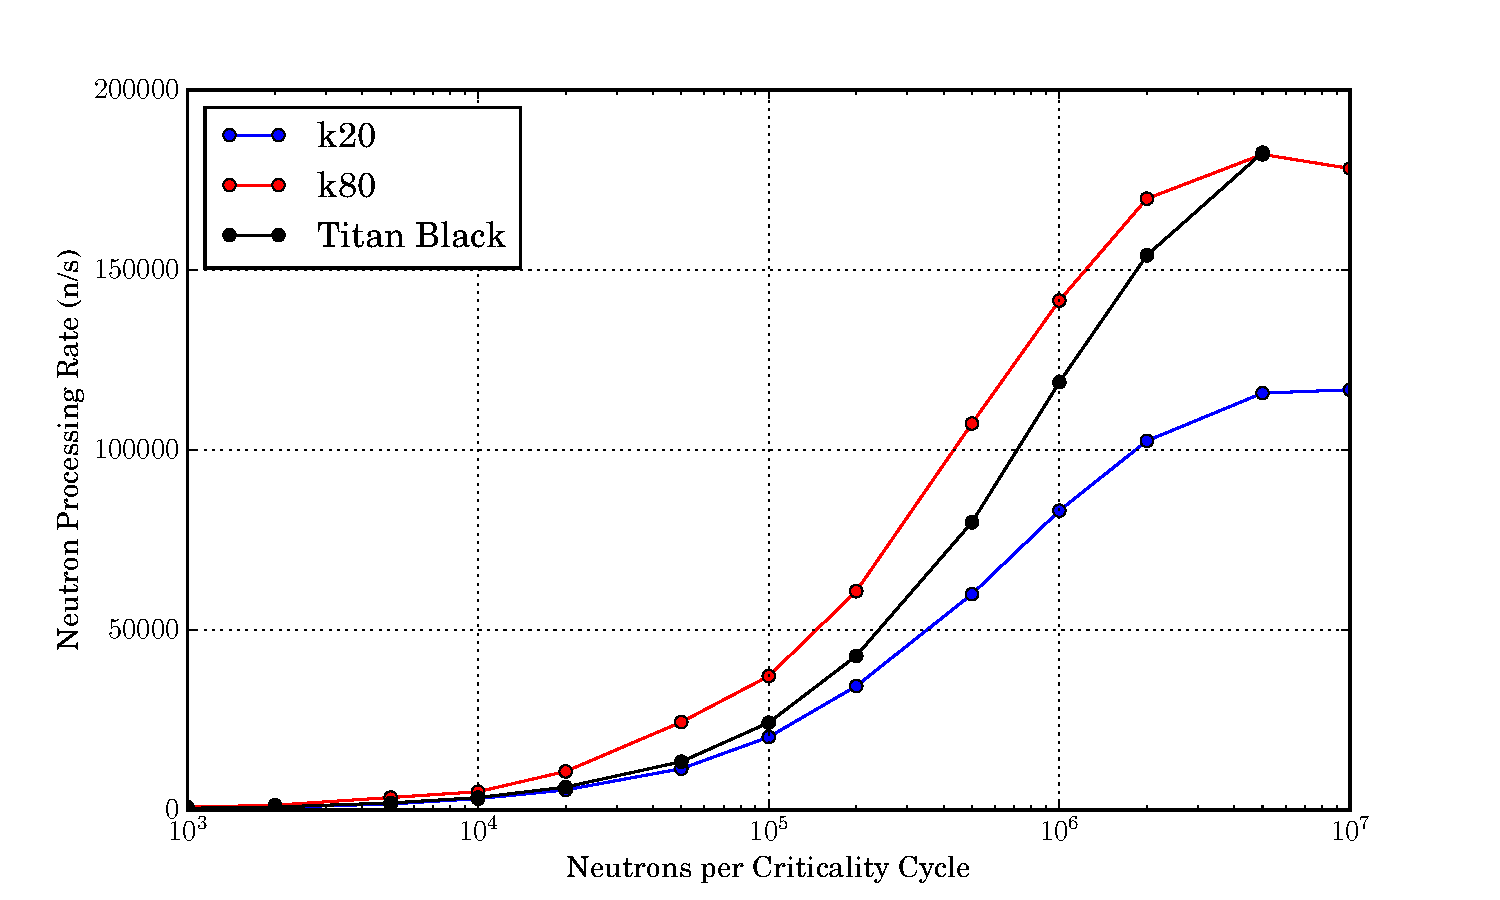
\includegraphics[width=0.8\textwidth,trim= 1cm 0cm 1cm 0cm]{graphics/scaling.pdf}
\caption{Neutron processing rate vs.\ number of neutrons per cycle for the hexagonal lattice test case. \label{scaling} }
\end{figure}

Performance increases until about $5\times10^6$ neutrons per cycle, then flattens above this for all cards.  This curve was calculated using the hexagonal pin lattice test case, and may change if a different model were input.  
% Is there a one-sentence argument for why this is reasonably representative or a good choice? Or, was it selected at random? coin toss?
Despite this, $5\times10^6$ neutrons per cycle is a rough estimate of where maximum performance occurs for WARP, and $6.5\times10^6$ neutrons per cycle was used for the test cases. 

\subsection{Multiplication Factors}

Table \ref{results_table_keff} shows the multiplication factor deviations for the six criticality tests compared to MCNP 6.1 and Serpent 2.1.24 for WARP running on an NVIDIA Titan Black, K20, and K80 cards.  The ``$\Delta$MCNP'' rows contains WARP's difference (in PCM) from MCNP, and the ``$\Delta$ Serpent'' rows contains WARP's difference from Serpent.  These difference rows also contain $1\sigma$ and $2\sigma$ values that indicate the level at which the multiplication factors calculated by WARP agree with either Serpent or MCNP.  A ``y'' in the $1\sigma$ position indicates that the multiplication factor values are mutually within 1 standard deviation of each other, i.e.\ that $\Delta \textrm{MCNP}<\sigma_{\textrm{MCNP}}+\sigma_{\textrm{WARP}}$.  This is the 90\% confidence interval and there is a 10\% probability that the the two codes could produce results outside of this interval.  The $2\sigma$ position is simply double the $1\sigma$ width and corresponds to the 99.8\% confidence interval (0.2\% chance of being outside).
% I think those confidence interval numbers oringinally here are wrong: https://en.wikipedia.org/wiki/68%E2%80%9395%E2%80%9399.7_rule
% Oh, maybe I'm misunderanding. This is the sigma interval overlaps? You might want to specify more conretely or add a citation b/c I think a lot of engineers use this idea incorrectly.


\begin{table}[h]
\centering
\caption{The test case multiplication factors for WARP versus those of Serpent 2.1.24 and MCNP 6.1.}
\label{results_table_keff}
\scriptsize
\begin{tabular}{| l | r | r | r |}
\cline{2-4}
\multicolumn{1}{c|}{}               & Jezebel                         &  Homogenized Block               & Pin Cell                          \\
\hline                          
Serpent 2.1.24                      & 0.9997840 $\pm$ 9.50E-5         & 0.5934090 $\pm$ 1.20E-4          & 0.2750510 $\pm$ 1.80E-4           \\
\hline                          
MCNP 6.1                            & 0.9999600 $\pm$ 7.00E-5         & 0.5933000 $\pm$ 4.00E-5          & 0.2751700 $\pm$ 7.00E-5           \\
\hline                          
WARP Titan Black                    & 1.0000620 $\pm$ 9.58E-5         & 0.5933724 $\pm$ 1.24E-4          & 0.2750294 $\pm$ 1.46E-4           \\
    \qquad\qquad   $\Delta$ Serpent & 27.80, $1\sigma$ n, $2\sigma$ y & -3.66, $1\sigma$ y, $2\sigma$ y  &  -2.16, $1\sigma$ y, $2\sigma$ y  \\
    \qquad\qquad   $\Delta$ MCNP    & 10.20, $1\sigma$ y, $2\sigma$ y &  7.24, $1\sigma$ y, $2\sigma$ y  & -14.06, $1\sigma$ n, $2\sigma$ n  \\
\hline
WARP K20                            & 1.0000212 $\pm$ 7.82E-5         & 0.5934539 $\pm$ 1.66E-4          & 0.2751048 $\pm$ 2.07E-4           \\
    \qquad\qquad   $\Delta$ Serpent & 23.72, $1\sigma$ n, $2\sigma$ y & 4.49 , $1\sigma$ y, $2\sigma$ y  &   5.38, $1\sigma$ y, $2\sigma$ y  \\
    \qquad\qquad   $\Delta$ MCNP    &  6.12, $1\sigma$ y, $2\sigma$ y & 15.39, $1\sigma$ n, $2\sigma$ y  &  -6.52, $1\sigma$ y, $2\sigma$ y  \\
\hline
WARP K80                            & 0.9999602 $\pm$ 9.58E-5         & 0.5932266 $\pm$ 1.24E-4          & 0.2749884 $\pm$ 1.56E-4           \\
    \qquad\qquad   $\Delta$ Serpent & 17.62, $1\sigma$ y, $2\sigma$ y & -18.24, $1\sigma$ n, $2\sigma$ y &  -6.36, $1\sigma$ y, $2\sigma$ y  \\
    \qquad\qquad   $\Delta$ MCNP    &  0.02, $1\sigma$ y, $2\sigma$ y &  -7.34, $1\sigma$ y, $2\sigma$ y & -18.26, $1\sigma$ n, $2\sigma$ n  \\
\hline
\end{tabular}

\smallskip

\begin{tabular}{| l | r | r | r |}
\cline{2-4}
\multicolumn{1}{c|}{}               & FLiBe Cell                      & Sodium Pin Cell                  & Hex Assembly                      \\
\hline                       
Serpent 2.1.24                      & 0.8804900 $\pm$ 8.70E-5         & 1.0987100 $\pm$ 2.20E-4          & 1.0503300 $\pm$ 7.20E-5           \\
\hline                       
MCNP 6.1                            & 0.8805100 $\pm$ 6.00E-5         & 1.0987700 $\pm$ 6.00E-5          & 1.0506500 $\pm$ 9.00E-5           \\
\hline                       
WARP Titan Black                    & 0.8807005 $\pm$ 9.58E-5         & 1.0986860 $\pm$ 7.82E-5          & 1.0510795 $\pm$ 9.58E-5           \\
    \qquad\qquad   $\Delta$ Serpent & 21.05, $1\sigma$ n, $2\sigma$ y & -2.40, $1\sigma$ y, $2\sigma$ y  &  74.95, $1\sigma$ n, $2\sigma$ n  \\
    \qquad\qquad   $\Delta$ MCNP    & 19.05, $1\sigma$ n, $2\sigma$ y & -8.40, $1\sigma$ y, $2\sigma$ y  &  42.95, $1\sigma$ n, $2\sigma$ n  \\
\hline
WARP K20                            & 0.8807086 $\pm$ 9.58E-5         & 1.0987912 $\pm$ 5.53E-5          & 1.0510620 $\pm$ 9.58E-5           \\
    \qquad\qquad   $\Delta$ Serpent & 21.86, $1\sigma$ n, $2\sigma$ y & 8.12, $1\sigma$ y, $2\sigma$ y   &  73.20, $1\sigma$ n, $2\sigma$ n  \\
    \qquad\qquad   $\Delta$ MCNP    & 19.86, $1\sigma$ n, $2\sigma$ y & 2.12, $1\sigma$ y, $2\sigma$ y   &  41.20, $1\sigma$ n, $2\sigma$ n  \\
\hline
WARP K80                            & 0.8807546 $\pm$ 9.58E-5         & 1.0985898 $\pm$ 5.53E-5          & 1.0511035 $\pm$ 1.24E-4          \\
    \qquad\qquad   $\Delta$ Serpent & 26.56, $1\sigma$ n, $2\sigma$ y & -12.02, $1\sigma$ y, $2\sigma$ y &  77.35, $1\sigma$ n, $2\sigma$ n  \\
    \qquad\qquad   $\Delta$ MCNP    & 24.56, $1\sigma$ n, $2\sigma$ y & -18.02, $1\sigma$ y, $2\sigma$ y &  45.35, $1\sigma$ n, $2\sigma$ n  \\
\hline
\end{tabular}
\end{table}


From Table \ref{results_table_keff}, it can be seen that WARP agrees with either MCNP \emph{or} Serpent (they sometimes do not exactly agree with each other!) at the $1\sigma$ level for all cases except the FliBe cell and the hex assembly cases.  The FliBe cell case agrees on the $2\sigma$ level, but the hex assembly case does not, indicating that there is a problem with the way WARP is solving the hex assembly case.  Speculation on what could be causing this is discussed in Section \ref{sec:disc}.


\subsection{Runtimes}
Table \ref{results_table_times} shows the transport cycle runtimes for the six criticality tests compared to MCNP 6.1 and Serpent 2.1.24 for WARP running on an NVIDIA Titan Black, K20, and K80 cards.  The values in the time rows are reported in minutes.  The ``$\Delta$ MCNP'' row contains WARP's speedup factor over MCNP, and the ``$\Delta$ Serpent'' row contains WARP's speedup factor over Serpent.


\begin{table}[h]
\centering
\caption{The test case transport cycle run times (in minutes) for WARP, Serpent 2.1.24, and MCNP 6.1.  Values in the ``$\Delta$'' rows contain the speedup factor of WARP compared the the corresponding production code running on a Berkelium (Bk) PSSC node and a Savio2 node.}
\label{results_table_times}
\scriptsize
\begin{tabular}{| l r | r | r | r |}
\cline{3-5}
\multicolumn{2}{c|}{}                            & Jezebel     & Homogenized Block & Pin Cell     \\
\hline                          
Serpent 2.1.24   &    Bk PSSC                    & 7.24        & 39.41             & 146.15       \\
                 &    Savio2                     & 6.32        & 24.10             & 76.51        \\
\hline                                        
MCNP 6.1         &    Bk PSSC                    &  30.57      & 98.40             & 131.27       \\
                 &    Savio2                     &   4.95      & 44.03             & 64.18        \\
\hline                          
\multicolumn{2}{|l|}{WARP Titan Black}           &  1.47       & 7.53              &  26.47       \\
\multicolumn{2}{|r|}{$\Delta$ Serpent (Bk, S2)}  & 4.91  4.29  & 5.23  3.20        &  5.52  2.89  \\
\multicolumn{2}{|r|}{$\Delta$ MCNP    (Bk, S2)}  & 20.74 3.36  & 13.07 5.85        &  4.96  2.42  \\
\hline
\multicolumn{2}{|l|}{WARP K20}                   & 2.45         & 12.60            & 42.55        \\
\multicolumn{2}{|r|}{$\Delta$ Serpent (Bk, S2)}  & 2.96  2.58   & 3.13  1.91       & 3.44  1.80   \\
\multicolumn{2}{|r|}{$\Delta$ MCNP    (Bk, S2)}  & 12.49 2.02   & 7.81  3.50       & 3.09  1.51   \\
\hline
\multicolumn{2}{|l|}{WARP K80}                   & 1.18         & 5.79             & 20.91        \\
\multicolumn{2}{|r|}{$\Delta$ Serpent (Bk, S2)}  & 6.11  5.34   & 6.81  4.17       & 6.99  3.66   \\
\multicolumn{2}{|r|}{$\Delta$ MCNP    (Bk, S2)}  & 25.80 4.18   & 17.01 7.61       & 6.28  3.07   \\
\hline
\end{tabular}

\smallskip

\begin{tabular}{| l r | r | r | r |}
\cline{3-5}
\multicolumn{2}{c|}{}                            & FLiBe Cell   & Sodium Pin Cell & Hex Assembly  \\
\hline                                    
Serpent 2.1.24   &   Bk PSSC                     & 79.16        & 120.86          & 81.54         \\
                 &   Savio2                      & 45.08        &  68.46          &  44.32        \\
\hline                                        
MCNP 6.1         &   Bk PSSC                     & 269.47       & 320.40          & 160.68        \\
                 &   Savio2                      & 81.03        & 199.15          & 112.25        \\
\hline                       
\multicolumn{2}{|l|}{WARP Titan Black }          &  25.78       & 81.18           & 34.91         \\
\multicolumn{2}{|r|}{$\Delta$ Serpent (Bk, S2)}  &  3.07  1.75  & 1.49  0.84      & 2.34  1.27    \\
\multicolumn{2}{|r|}{$\Delta$ MCNP    (Bk, S2)}  &  10.45 3.14  & 3.95  2.45      & 4.60  3.22    \\
\hline
\multicolumn{2}{|l|}{WARP K20 }                  & 39.83        & 121.34          & 56.03         \\
\multicolumn{2}{|r|}{$\Delta$ Serpent (Bk, S2)}  &  1.99  1.13  & 1.00  0.56      & 1.46  0.79    \\
\multicolumn{2}{|r|}{$\Delta$ MCNP    (Bk, S2)}  &  6.77  2.03  & 2.64  1.64      & 2.87  2.00    \\
\hline
\multicolumn{2}{|l|}{WARP K80   }                & 24.68        & 81.40           & 35.63         \\
\multicolumn{2}{|r|}{$\Delta$ Serpent (Bk, S2)}  & 3.21  1.83   &  1.48  0.84     &  2.29  1.24   \\
\multicolumn{2}{|r|}{$\Delta$ MCNP    (Bk, S2)}  & 10.92 3.28   &  3.94  2.45     &  4.51  3.15   \\
\hline
\end{tabular}
\end{table}


It can be seen from Table \ref{results_table_times} that WARP runs fastest on the K80 card, and both Serpent and MCNP run fastest on the Savio2 node.  This makes sense since these are the two newest pieces of hardware considered.  It is important to note that the Titan Black card performs almost as well as the K80 card, however.  Comparing the K80 card to a Savio2 node (the most relevant comparison), WARP runs 0.84 to 5.34 times as fast as Serpent and 2.45 to 7.61 times as fast as MCNP.   The largest speedup over Serpent is for the Jezebel test, the largest speedup over MCNP is for the homogenized block test, and the smallest speedup is for the sodium pin cell test over both Serpent and MCNP.  This speedup factor is calculated over an entire compute node, so WARP on a GPU gives a performance equivalent to 0.84 to 7.61 compute nodes, depending on the type of simulation hardware considered.  For the sodium pin case, where there is a relatively large amount of cross section processing, a Savio2 node running Serpent actually performs better than WARP on a K80 card.  For problems where there is less cross section processing (higher geometry processing fraction), WARP tends to perform better than a Savio2 node running Serpent.  WARP always performs better than a Savio2 node running MCNP, even with relatively heavy cross section processing, but this isn't a great surprise considering that MCNP doesn't use a unionized energy grid structure when processing cross sections.


\subsection{Spectra}

In the following subsections, spectra calculated by WARP are compared to those calculated by Serpent and MCNP for identical geometries and materials.  Every spectrum is binned into 1024 equi-log bins from $10^{-11}$ to $20$ MeV.  In tests where there is a large region of little to no flux (like in the fast spectrum inside the Jezebel sphere), the energy bin structure is not changed, but the energy range of the plot is limited to the region where there is nonzero flux.  The relative difference compared to the MCNP spectrum is shown in the top subplot below the main spectrum plot, and the relative difference from the Serpent spectrum is shown in the lower subplot.  The green shaded area in the error subplots shows the space within 2 standard deviations of the statistical uncertainty of the production code.  Unlike the intervals reported in the previous subsection, the interval shown in green is only for the production code results.  In other words, the codes should have results within the 2$\sigma$ interval 95.45\% of the time (as opposed to 99.8\% of the time).

%%%%%
\newpage
\subsubsection{Test 1 - ``Jezebel'' Bare Pu Sphere}

Figure \ref{jezebel_spec} shows the volume-averaged flux spectra in the Jezebel sphere.  The relative difference of WARP compared to Serpent and MCNP is very low, with the normalized tally bins being less than 0.5\% from each other in regions where the flux is large.  Of course, when the flux is small, the statistical uncertainty becomes much higher, and the relative difference becomes noisy.   The relative error is almost always inside the 2$\sigma$ confidence interval as well, indicating that the simulations are statistically identical. 

\begin{figure}[h!]
\centering
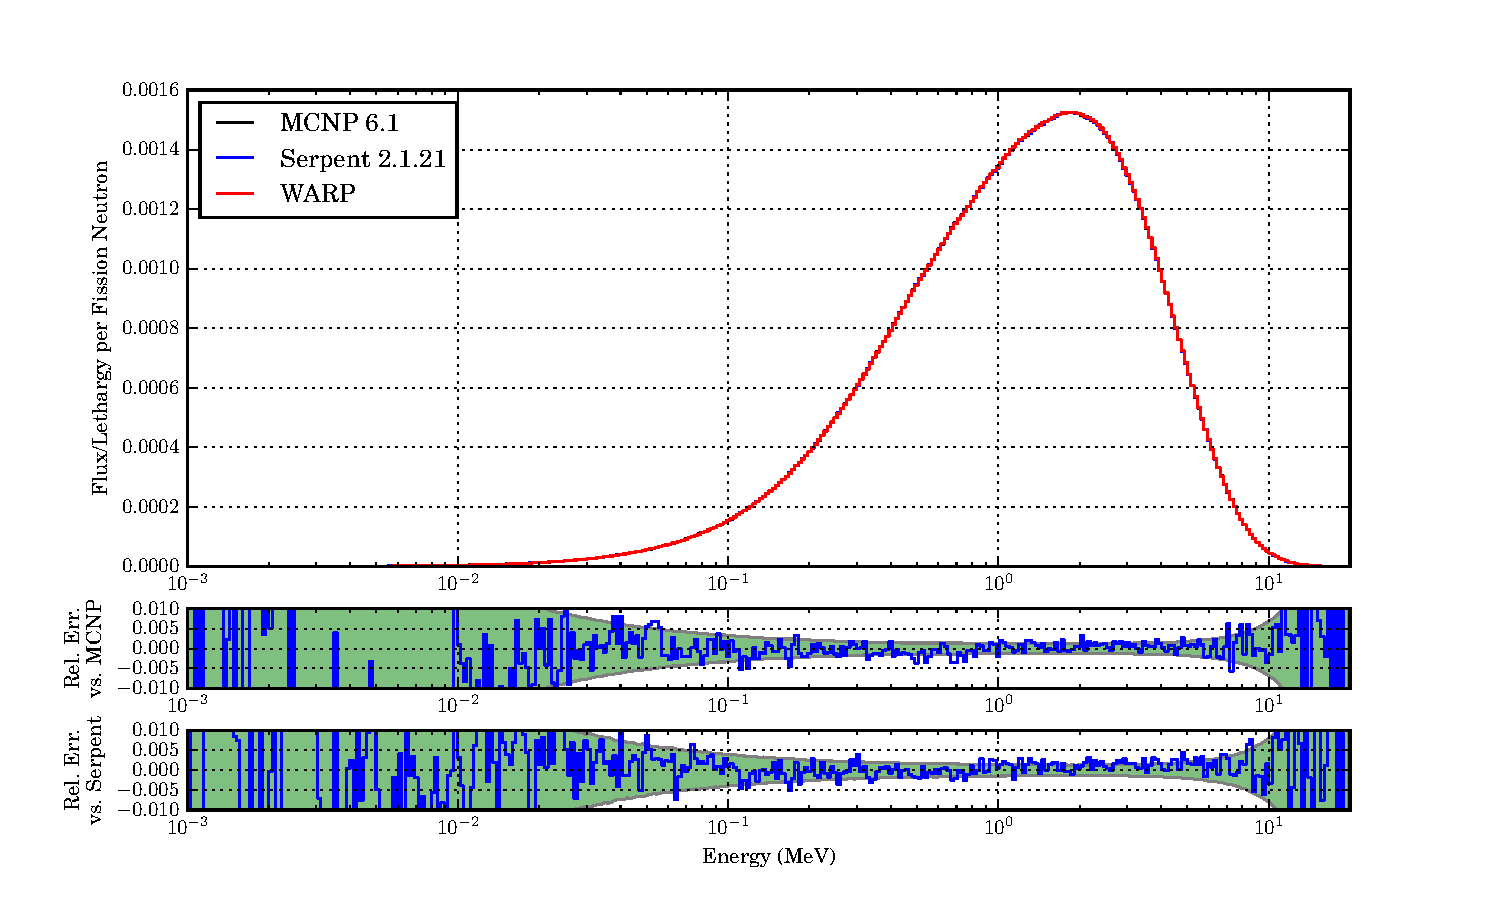
\includegraphics[width=0.9\textwidth,trim= 1cm 0cm 1cm 0cm]{graphics/jezebel_spec.pdf}
\caption{Volume-averaged flux spectra inside the sphere of the Jezebel test case. \label{jezebel_spec} }
\end{figure}

%%%%%
\newpage
\subsubsection{Test 2 - Homogenized Fuel Block}

Figure \ref{homfuel_spec} shows the volume-averaged flux spectra in the homogenized fuel block.  The relative difference compared to MCNP and Serpent is again shown in the lower subplots.  The relative difference compared to MCNP is again generally less than 0.15\% and appears to have a zero mean, but the error compared to Serpent has a constant positive offset, indicating a slightly different normalization.  This kind of offset appears in other spectra as well, but only when comparing to Serpent.  This indicates a possible normalization discrepancy between MCNP and Serpent.  There also appears to be some  deviations with similar structure from 0.1 to 0.3 MeV, indicating that some kind of reaction sampling may not be treated exactly the same way as in Serpent and MCNP.

\begin{figure}[h!]
\centering
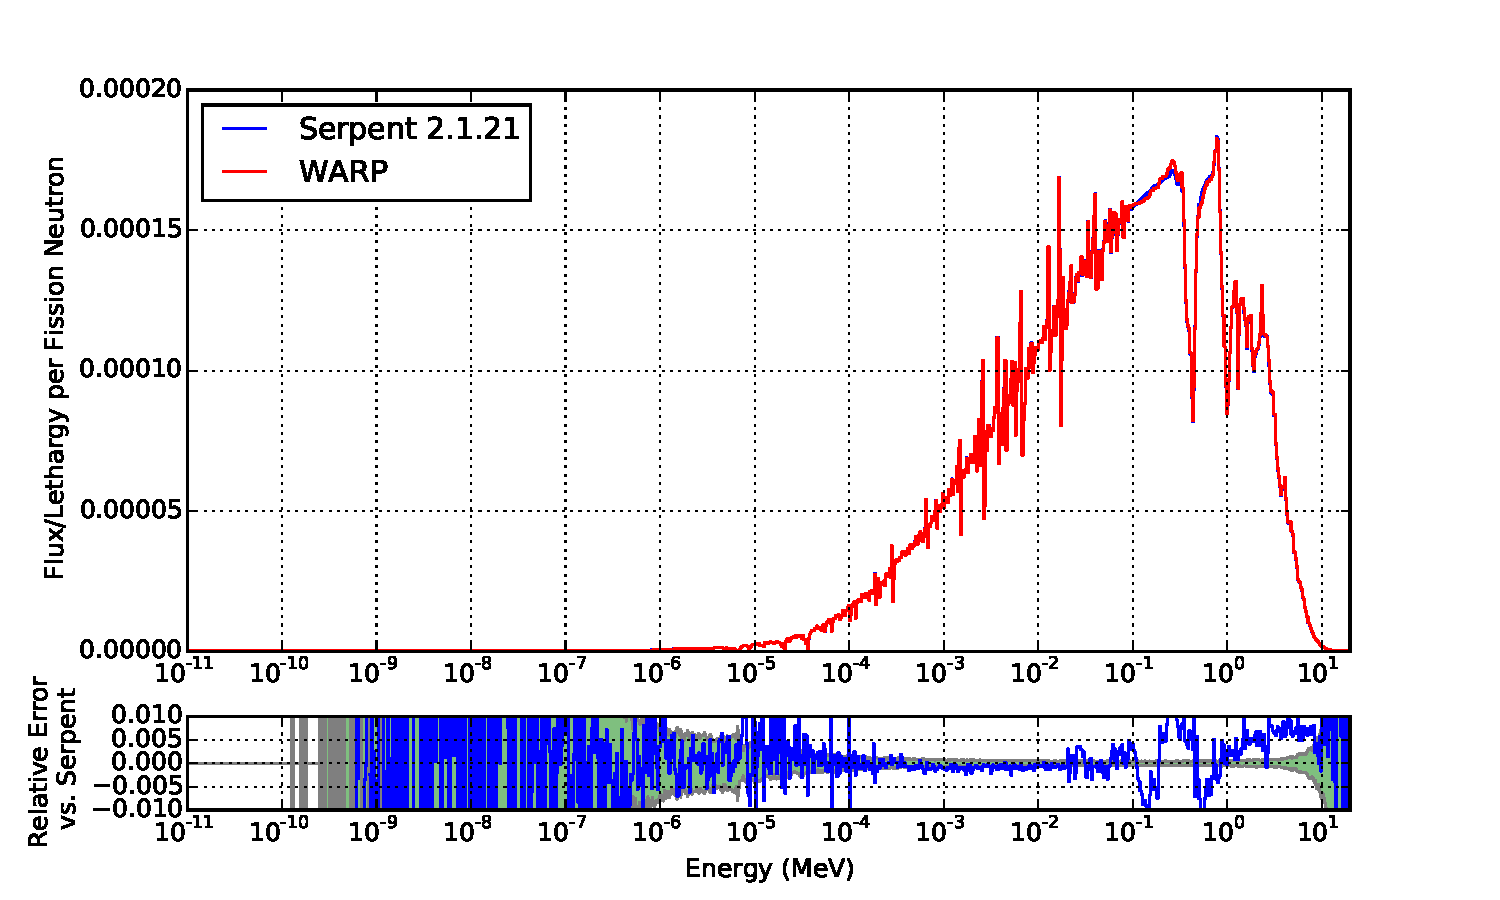
\includegraphics[width=0.9\textwidth,trim= 1cm 0cm 1cm 0cm]{graphics/homfuel_spec.pdf}
\caption{Volume-averaged flux spectra inside the homogenized fuel block. \label{homfuel_spec} }
\end{figure}

%%%%%
\newpage
\subsubsection{Test 3 - Zr-Clad UO$_2$ Pin in Heavy Water}

Figure \ref{pincell_spec} shows the volume-averaged flux spectra inside the fuel rod in the Zr-clad UO$_2$ pin in the heavy water test case.  Again, the relative difference is generally less than 1\% where the flux is large.  Compared to Serpent, the WARP spectrum again appears to have a small, constant offset.  The entire energy range agrees well with MCNP, however, indicating that all the reaction laws were processed identically to MCNP for the nuclides present in this test case.
% in the previous case it was 0.15%; before that you didn't mention a number, now it's 1. I'd explicitly differentiate between confidence interval and rel err, because the use of percentages in both cases could be misleading. 


\begin{figure}[h!]
\centering
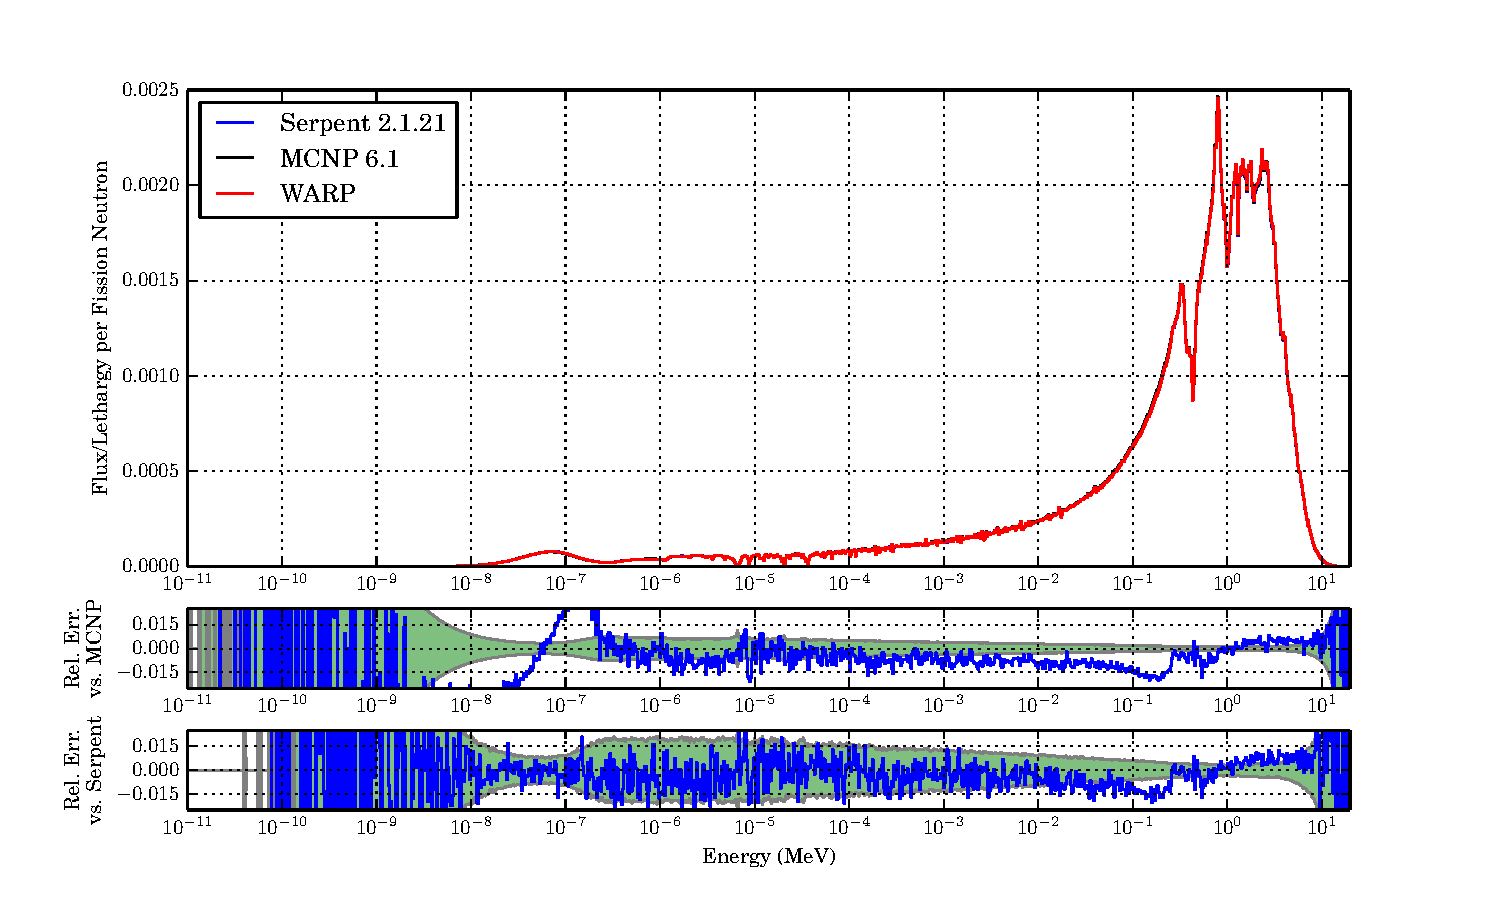
\includegraphics[width=0.9\textwidth,trim= 1cm 0cm 1cm 0cm]{graphics/pincell_spec.pdf}
\caption{Volume-averaged flux spectra inside the oxide fuel of the Zr-clad pin in the pin in heavy water test case. \label{pincell_spec} }
\end{figure}

%%%%%
\newpage
\subsubsection{Test 4 - Homogenized Fuel Pebble in FLiBe}

Figure \ref{flibe_spec} shows the volume-averaged flux spectra in the fuel pebble for the reflective FLiBe test case.  Here, the relative difference is generally less than 0.1\% where the flux is large.  The WARP spectrum again has a constant offset compared to the Serpent spectrum, but compares well to MCNP apart from the significant deviations around large resonances in the 20 keV to 1 MeV range.  

\begin{figure}[h!]
\centering
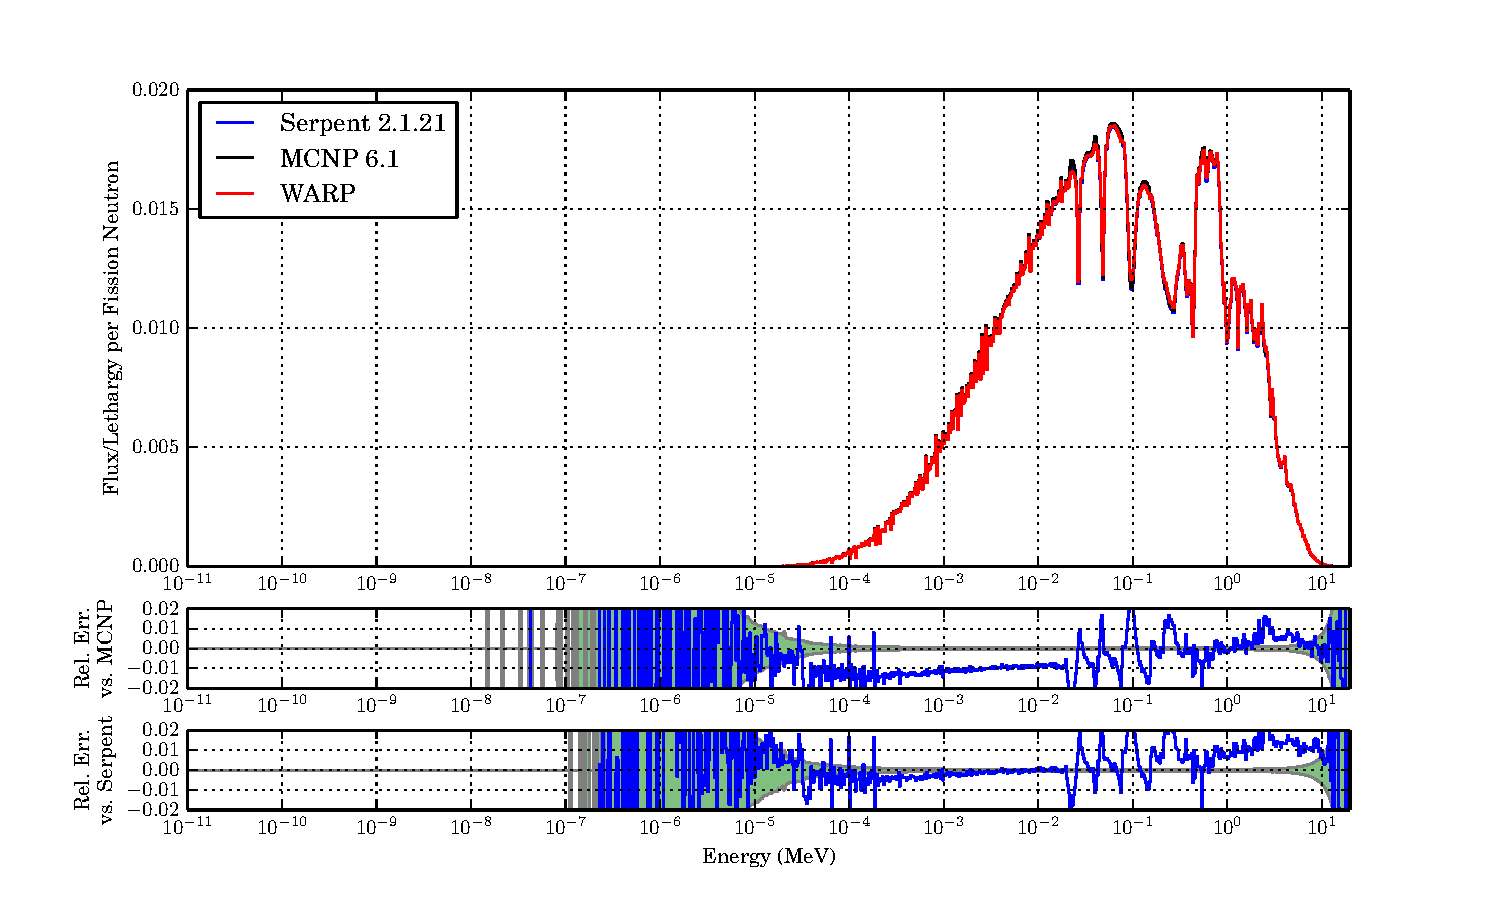
\includegraphics[width=0.9\textwidth,trim= 1cm 0cm 1cm 0cm]{graphics/flibe_spec.pdf}
\caption{Volume-averaged flux spectra inside the fuel pebble of the reflective FLiBe test case. \label{flibe_spec} }
\end{figure}

%%%%%
\newpage
\subsubsection{Test 5 - Stainless Steel Clad Metallic Uranium Pin in Liquid Sodium}

Figure \ref{sodiumpin_spec} shows the volume-averaged flux spectra in the fuel for the reflective sodium cooled, steel clad, metallic fuel test case.  The relative difference is generally less than 0.1\% where the flux is large.  The WARP spectrum again has a constant offset compared to the Serpent spectrum, but compares well to MCNP apart from the significant deviations around large resonances in the 20 keV to 1 MeV range.  This again highlights that there is probably a reaction law that isn't processed identically to MCNP.

\begin{figure}[h!]
\centering
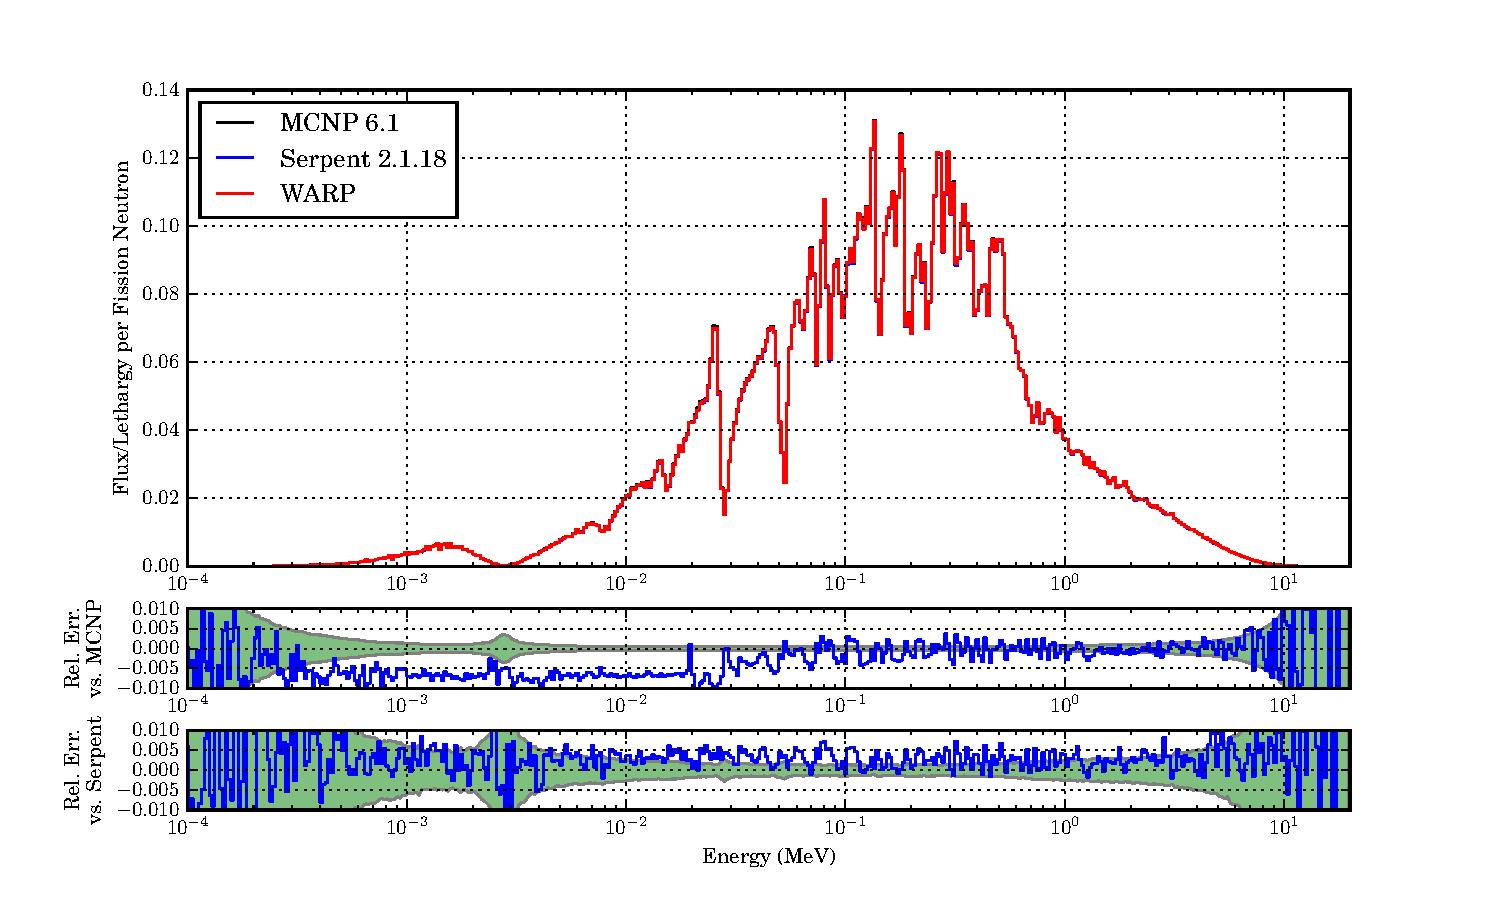
\includegraphics[width=0.9\textwidth,trim= 1cm 0cm 1cm 0cm]{graphics/sodiumpin_spec.pdf}
\caption{Volume-averaged flux spectra inside the fuel of the reflective, steel clad, sodium cooled pin test case. \label{sodiumpin_spec} }
\end{figure}


%%%%%
\newpage
\subsubsection{Test 6 - Zr-Clad Hexagonal UO$_2$ Pin Cell Lattice in Light Water}

Figure \ref{assembly-lw_spec} shows the volume-averaged flux spectrum in the center pin of the Zr-clad hexagonal oxide fuel pin lattice in light water test case. The relative difference is generally less than 5\% where the flux is large, but this time the WARP results are always within the statistical error of both MCNP and Serpent.  There is no constant offset compared to Serpent or MCNP and no large deviations, indicating that all the reaction laws were processed identically to both Serpent and MCNP for the nuclides present in this test case.  This is also the only test case other than Jezebel where MCNP and Serpent give identical spectra.

\begin{figure}[h!]
\centering
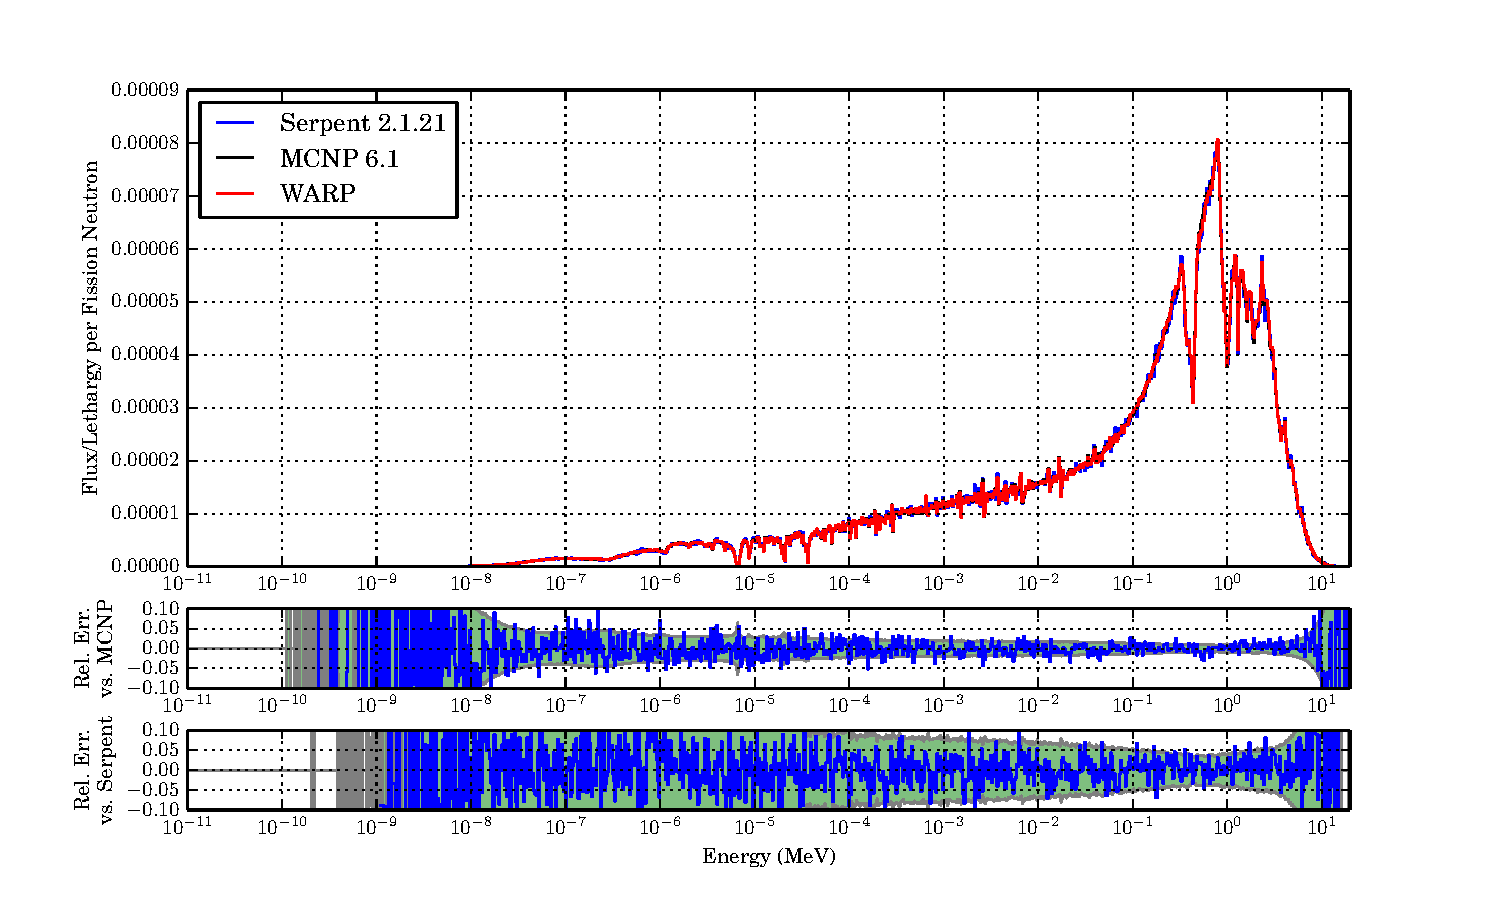
\includegraphics[width=0.9\textwidth,trim= 1cm 0cm 1cm 0cm]{graphics/assembly-lw_spec.pdf}
\caption{Volume-averaged flux spectra inside the center fuel pin of the hexagonal pin lattice test case. \label{assembly-lw_spec} }
\end{figure}

\newpage
\subsection{History Power}

For productivity, the ``history power,'' or  number of neutron histories processed per unit time, is of primary interest when purchasing a system since it determines how quickly results can be produced.  In addition to this, the history power per hardware cost is of interest for initial capital investment, and the history power per unit energy is of interest for operational costs.  Table \ref{history_power} shows the history power and relative costs of GPU systems running WARP compared to MCNP and Serpent running on a the aforementioned CPU platforms.  

\begin{table}[h]
\centering
\caption{The history power and costs of performing Monte Carlo neutron transport on GPU and CPU systems.}
\label{history_power}
\small
\begin{tabular}{| l r | r | r | r |}
\cline{3-5}
\multicolumn{2}{c|}{}             & H. Power   & H.P. / Capital   & H.P. / watt  \\
\hline                            
Serpent 2.1.24   &   Bk PSSC      & 2.32E+6    &   249           &  5,033        \\
                 &   Savio2       & 8.84E+6    & 1,305           & 42,082        \\
\hline                                 
MCNP 6.1         &   Bk PSSC      & 2.32E+6    &   249           &  5,033        \\
                 &   Savio2       & 4.63E+6    &   684           & 22,039        \\
\hline                            
WARP             &   Titan Black  & 1.32E+7    & 8,675           & 52,778        \\
                 &   K20          & 8.52E+6    & 2,561           & 37,847        \\
                 &   K80          & 1.38E+7    & 2,760           & 45,995        \\
\hline
\end{tabular}
\end{table}
% I'd put the /Capital in units. Is it $ or cents?

The history powers shown in Table \ref{history_power} were calculated by summing the total number of neutrons processed in all six test cases and dividing this number by the sum of the runtimes of the six cases for each code/platform combination (i.e.\ $3.9\times10^8 / \textrm{sum of run times}$).  This way, the average is not biased towards a special case that allows a code to process neutrons especially quickly.  The history power per capital is simply the averaged neutron processing rate divided by the hardware cost of the platform.  The history power per watt is similar, except divided by the platform's total maximum electrical power consumption rather than the cost.  The costs and electrical power consumptions used to calculate these values were shown in Table \ref{platform_table}.


Table \ref{history_power} shows that, on average, for the test cases considered, a new NVIDIA GPU card can process neutrons about 1.6 times as fast as a new multiprocessor/multicore CPU node running Serpent and about 3 times as fast as a CPU node running MCNP.  From a capital investment standpoint, the a K80 card costs about half as much as a Savio2 node per neutron processing power and consumes about the same amount of electricity.  The Titan Black, however, performs about as well as a K80 from the neutron processing rate standpoint, but costs about a third as much and consumes 20\% less electricity.  Since WARP uses single-precision data and math in order to fully exploit the capabilities available on consumer GPUs (like the Titan Black), the capital and electrical costs of running WARP can be greatly reduced. 
% I don't understand the logical connection of this last sentence. Reduced by doing what?  


%%%%%%%%%%%%%%%%%%%
%%%%%%%%%%%%%%%%%%%
%%%%%%%%%%%%%%%%%%%

\section{Discussion}
\label{sec:disc}

The differences seen in the multiplication factors and spectra calculated by WARP compared to those calculated by Serpent and MCNP are most likely due to either a reaction law being inexactly processed or reaction types being slightly incorrectly sampled.  Whether this is due to a software ``bug'',
% you might want to include a footnote or something discussing the test framework, or an appendix about what has been tested. This sentence just seems a little "well, our code might be wrong. idk". 
 or if it has to do with single precision math has not been determined.  Some laws potentially require division by small numbers then comparing or adding the result to other numbers.  Roundoff error from single precision math could make these operations inaccurate and ultimately lead to visible differences in the neutron spectra and multiplication factor.  

Monte Carlo is a great place to take advantage of single precision math since solution convergence does not normally depend on derivatives, except perhaps in a cross section processing law, and the calculated results are typically not required to be more precise than single-precision numbers.  The major places roundoff error can affect the solution is in tally accumulation and cross section processing.  Currently, WARP calculates the total macroscopic cross section of a material on the fly, and roundoff could become a problem around resonances where the cross section of one nuclide (or several) is much larger than the that of the other nuclides in the material.  In this case, the additions from the minor cross section nuclides could be neglected and could lead to oversampling their reactions in the subsequent routines (since the material's calculated total macroscopic cross section would be smaller than it should be).  This problem could be circumvented by preprocessing the material's total macroscopic cross section using double precision math on the host before the data is given to the GPU as single precision numbers.  This, however, would increase the memory footprint of the data.

Another place roundoff error could cause problems is in tally accumulation.  WARP calculates the flux in a cell by calculating the inverse of the macroscopic cross section at a collision site and adding it to the sum of all previous collisions.  If a large resonance lies within an energy bin, very dissimilar values could be added together and precision could be lost.  This could be circumvented by using double precision data for the tally arrays.  The cost of doing so would have to be measured, but hopefully it would be small since tally accumulation only happens once per transport cycle and is therefore a relatively infrequent operation.

WARP uses integer math to calculate multiplication factors.  Long integer values for the total number of fissions produced in a simulation are stored on the host, and integer yield values from each batch are accumulated into it.  At the end of the simulation, the long integer value containing the total number of fission neutrons produced is divided by the total number of source neutrons run, yielding the final value for the multiplication factor. Since integer math is used during this whole process, roundoff error from accumulation can not affect it as long as overflow doesn't occur (hence using the long integer data type).  Roundoff error in the reaction selection and processing routines could affect the individual yield values and their frequency, however.

It is worth noting that MCNP and Serpent calculated somewhat different solutions in these studies, which shows that getting exactly the same answer is quite difficult since each code handles things slightly differently.  This makes it difficult to know what is really correct, but as long as the results are under the error level of what can be detected in the physical world, any differences in the codes should be irrelevant.  One potential niche use for WARP would be to do cheap and fast calculations where large total throughput is needed, not precision.  For example, in a large parametric study, once an optimal region has been found in the parameter space, WARP's job would be done.  This knowledge could then be used as a starting point for more precise calculations with CPU codes.

% This is a good thought. You might want to break this into two paragraphs and expand the second one to include a few more ideas. You might also discuss if there are places that a conventional code could do parts of the calcualtion with warp, or warp-like algorithms...


%%%%%%%%%%%%%%%%%%%
%%%%%%%%%%%%%%%%%%%
%%%%%%%%%%%%%%%%%%%
\section{Conclusions and Future Development}
\label{sec:concdev}

It has been shown that WARP is able to accelerate high-fidelity neutron transport on GPUs.  Depending on the problem type and the card used, WARP can achieve performance equivalent to that of 0.84 to 7.61 modern CPU nodes on a single GPU card, depending on the CPU code and type of calculation being considered.  The low capital and electrical cost of GPU platforms then lead to about 2 to 3 times more histories calculated per dollar spent.  This clearly shows that GPUs can be very cost effective for continuous energy Monte Carlo neutron transport.  This efficiency comes at the cost of precision, however, but WARP could still be a useful tool for scenarios where high computational throughput and/or low-cost calculations are of importance.

WARP, which is developmental, may still have some ``bugs'', as evidenced by the slight deviations of the multiplication factors and spectra compared to MCNP and Serpent.  
% Again, perhaps note the test efforts.
A large part of future development will be eliminating these discrepancies.  The initial goals of WARP have been completed, but there is much work still to be done if it is going to be of real use to the nuclear engineering community.  Basic functionality is currently good enough to assure that GPUs can accelerate high-fidelity Monte Carlo neutron transport calculations, but many capabilities need to be expanded and ensured to scale well to large numbers of neutrons, isotopes, and geometric zones.  The rest of this section goes over the major areas where WARP could be improved in order to ensure good scaling in these dimensions.    

Geometry is currently handled by NVIDIA OptiX, which provides a convenient way to obtain high-performance results. However, OptiX had to be coerced into providing WARP with the extra information it needed beyond the distance to the nearest intersection, namely the material and tally indices.  The way OptiX is used to determine these numbers is not efficient since it must be done iteratively using OptiX's native functions instead of calculating the sum of surface normals in a single trace.  NVIDIA has released ``OptiX Prime'' with OptiX 3.5 \cite{optix3.5}, which promises to provide a more ``to the metal'' ray tracing experience, and might be leveraged to provide more efficient single-traverse functionality.  OptiX could also be replaced by Rayforce \cite{rayforce}, a high-performance GPU ray tracing library developed by VSL that has the desired functionality built-in and is currently available free of charge for noncommercial use.

The OptiX geometry routines could also be replaced by handwritten routines that use combinatorial solid geometry like Serpent and MCNP.  This would make writing input for WARP more like what most nuclear engineers are already used to and, more importantly, could provide a potential performance increase.  A universe-based CSG representation may map very well to the GPU and may even be able to fit inside of shared memory for small numbers of surfaces.  Using an efficient CSG method would further lend itself to using Woodcock delta-tracking for the neutrons and thus getting rid of the tracing algorithms and libraries altogether.   

WARP also suffers from ``tail effect,'' where performance drops off as the number of remaining active neutrons in a batch decreases \cite{algorithms}.  Developing a method that keeps the active neutron number high would greatly improve performance, but could become quite complicated as generations would start to overlap and calculation of the multiplication factor and converging the source distribution could not be done between cycles as it is now.  

If an entire overhaul of the WARP transport algorithm is feasible, using a streaming multiprocessor (SM)-based algorithm might be investigated for replacing the current global one.  This type of algorithm would treat each SM as an independent processor and would provide each a bank of neutrons to transport, as is done by Liu and Henderson \cite{tianyu,henderson}.   This way, neutron data could be stored in very fast shared memory, though this would compete with storing geometric information.  Also, since a smaller set of neutrons could be stored, the SMs would need to communicate to determine which of the next neutrons they would take out of the global bank, or they would need to periodically rendezvous to shared source information and ensure that the distributions they use are each converged.  This type of transport algorithm would also preclude using OptiX, since it does not have SM-level functionality \cite{optix}.

An efficient way to handle situations where there are many different material and isotopes present needs to be explored.  The work done by Scudiero on porting OpenMC's macroscopic cross section processing benchmarking tool, ``xsbench,'' may elucidate this endeavor \cite{openmc,scudiero}.   Since global memory comes at a premium on GPUs, an on-the-fly temperature treatment for nuclides would likely be required if more than a handful of isotopes are desired at more than one temperature.  Methods like those used in Serpent could be adapted for use on the GPU \cite{serpent}.  On-the-fly methods reduce the amount of storage needed, but they require more computation per data element loaded since the loaded value is adjusted according to the temperature of the material.  This kind of method may work well on the GPU since GPUs have a larger FLOP/byte ratio than CPUs and the additional work may cost little.  A grid thinning routine that discards closely-spaced energy grid points could also be added to WARP, saving memory but potentially costing accuracy.  Fractional cascading may also help reduce the memory footprint of the cross section data while keeping energy search cost low \cite{Lund2015}. 

WARP would gain usability if more features were incorporated as well.  Importance cutoffs could be used to terminate neutrons, leading to shorter runtimes; cell importances (easily attached to cell primitives), track length tallies, and implicit absorption could help improve tally statistics.  Developing an efficient way to include many reaction rate tallies would also make WARP useful for performing depletion analysis.  It would further be helpful for WARP to have statistical tests like Shannon entropy to ensure the fission source is fully converged before tallies and multiplication factors are accumulated.  Accuracy would also be improved by adding S($\alpha,\beta$) thermal scattering tables and unresolved resonance parameters.  Neutrons have statistical weight in WARP, so simple variance reduction techniques like implicit capture should be a straight-forward part of future development.  Path lengths are already calculated in OptiX, so implementing track length tallies could also be a straight-forward variance reduction technique to introduce into WARP.  Multi-GPU support should also be added so that WARP can be used effectively on computers with more than one GPU.

%Reproducibility of results when using the same random number seeds will also be investigated to ensure consistent results can be produced and that there are no systematic errors present in WARP.  Ensuring reproducibility will also be necessary in making a test suite for WARP, so future users can have confidence in their results and future developers can know their modifications do not introduce new errors into WARP.  

I'd include a summarizing paragraph here. It feels like a big laundry list of what's possible or what might make sense. Give us a quick reminder of what's unique, what you've accomplished, and results highlights. 

WARP will be released as open source software, pending DOE approval, at \url{http://github.com/weft}.  In a weave of cloth, The ``warp'' is the high-tension, longitudinal thread, whereas the ``weft'' is the low tension, transverse thread.  On a loom, the warp threads are all moved in sync, then the weft is passed through them.  Naming the repository for the single thread that defines the phase of the warp seemed appropriate.

\section*{Acknowledgements}
\label{sec:ack}

This research is based upon work partially supported by the U.S. Department of Energy National Nuclear Security Administration under Award Number DENA0000979 through the Nuclear Science and Security Consortium: http://nssc.berkeley.edu, as well as upon work supported under an Integrated University Program Graduate Fellowship.  This research also used the Savio computational cluster resource provided by the Berkeley Research Computing program at the University of California, Berkeley (supported by the UC Berkeley Chancellor, Vice Chancellor of Research, and Office of the CIO).

\section*{Disclaimer}
\label{sec:disc}

This report was prepared as an account of work sponsored by an agency of the United States Government. Neither the United States Government nor any agency thereof, nor any of their employees, makes any warranty, express or limited, or assumes any legal liability or responsibility for the accuracy, completeness, or usefulness of any information, apparatus, product, or process disclosed, or represents that its use would not infringe privately owned rights. Reference herein to any specific commercial product, process, or service by trade name, trademark, manufacturer, or otherwise does not necessarily constitute or imply its endorsement, recommendation, or favoring by the United States Government or any agency thereof. The views and opinions of authors expressed herein do not necessarily state or reflect those of the United States Government or any agency thereof.

\bibliographystyle{model1-num-names}
\bibliography{references}



\end{document}

